\documentclass[conference]{IEEEtran}

% ========================================================= 
% IDIOMA Y CODIFICACIÓN 
% ========================================================= 
\usepackage[utf8]{inputenc} 
\usepackage[T1]{fontenc} 
\usepackage[spanish,es-nodecimaldot]{babel} 

% ========================================================= 
% MATEMÁTICAS Y SÍMBOLOS 
% ========================================================= 
\usepackage{amsmath} 
\usepackage{amssymb} 

% ========================================================= 
% FIGURAS Y TABLAS (Compatibles con IEEEtran 2 columnas)
% ========================================================= 
\usepackage{graphicx} 
\usepackage{booktabs} 
\usepackage{array} 
\usepackage{tabularx}
\usepackage{stfloats}

% ========================================================= 
% LISTAS, CITAS E HIPERVÍNCULOS
% ========================================================= 
\usepackage{enumitem} 
\usepackage{cite} 
\usepackage[colorlinks=true, linkcolor=black, citecolor=black, urlcolor=black]{hyperref} 

% ========================================================= 
% INFORMACIÓN DEL DOCUMENTO 
% ========================================================= 
\title{\textbf{Caracterización y Detección de Antipatrones Arquitectónicos en Aplicaciones Basadas en IA Generativa y RAG}\\ \large Un estudio empírico} 
\author{\IEEEauthorblockN{Arlo Ocampo}} 

\begin{document}

\maketitle

% --- SECCIONES ---
\section{Introducción}
La Inteligencia Artificial Generativa y las arquitecturas de Retrieval-Augmented Generation (RAG) han adquirido una creciente relevancia en el desarrollo de aplicaciones de software, al permitir integrar modelos de lenguaje con componentes convencionales de recuperación, procesamiento y gestión de información. Esta integración introduce nuevas formas de interacción entre componentes de software que plantean desafíos para la calidad, mantenibilidad y evolución de las aplicaciones.

En este contexto, el presente anteproyecto, presentado ante el grupo de investigación SIGIIP, propone estudiar la presencia de antipatrones arquitectónicos en aplicaciones basadas en Inteligencia Artificial Generativa y RAG, con énfasis en su caracterización y detección mediante análisis estático. El documento presenta la selección y delimitación del tema, el planteamiento y formulación del problema, los objetivos, la justificación, el marco de referencia y las hipótesis de trabajo que orientan la investigación propuesta.
\section{Selección y Definición del Tema de Investigación}

El presenta trabajo de investigación sitúa dentro del área de \textbf{Arquitectura de software} y la \textbf{Ingeniería de Software empírica}, enfoncándose específicamente en los campos de calidad y mantenibilidad en sistemas basados en Inteligencia Artificial Generativa (GenAI) y Retrieved-Augmented Generation (RAG)

\subsection{Punto de Partida e Interés Temático}
Para la selección del tema, se parte desde interrogantes sobre la viabilidad y la relevancia de estudiar la degradación arquitectónica en aplicaciones de IA. Ante la creciente adopción de estos nuevos campos por parte de la industria, surgió la interrogante sobre si los errores en estas aplicaciones provienen exclusivamente del modelo o de la infraestructura de software. La revisión preliminar confirmó la existencia de información en repositorios de código abierto y literatura reciente \cite{shao_are_2024}, evidenciando que los resultados de esta investigación pueden aportar un marco de auditoria proactivo no presente en la actualidad.  

\subsection{Observación Directa y Consulta Bibliográfica}
A partir de la documentación en la literatura científica relacionada, se identificó el objeto de investigación: los defectos estructurales y anti-patrones de integración en aplicaciones RAG. Esta documentación permitió contrastar que, si bien existen taxonomías de fallos, la comunidad científica los aborda de manera reactiva \cite{shao_are_2024}.

\subsection{Delimitación y Definición del Tema}
Con el apoyo de la revisión bibliográfica y las directrices metodológicas del grupo de investigación MIS se delimitó el objeto de conocimiento. El tema central se define como la caracterización y detección estática de anti-patrones arquitectónicos en aplicaciones basadas en IA generativa y RAG, estableciendo el titulo preliminar del anteproyecto: \textbf{Caracterización y Detección de anti-patrones arquitectónicos en aplicaciones basadas en IA Generativa y RAG: Un estudio empírico}
\section{Problema de Investigación}
 
\subsection{Planteamiento del Problema}

La rápida adopción de la Inteligencia Artificial Generativa y la arquitecturas RAG ha transformado el desarrollo de software actual mediante la integración dinámica de modelos de lenguaje y bases vectoriales. Además de estar impulsadas por una intensa presión de mercado que ha relegado los estándares de calidad y ha normalizado malas practicas como código desordenado y prompts mezclados con la lógica de negocio \cite{shao_are_2024}.

De continuar sin intervención derivará en una deuda técnica creciente que solo revelará fallos críticos en producción y disparará los costos de mantenimiento. Problemática que este proyecto propone prever caracterizando dichos antipatrones y sentando bases metodológicas para el futuro desarrollo de una herramienta proactiva de análisis estático basada en arboles de sintaxis abstracta.
 
\subsection{Formulación del Problema}
 
¿De qué manera la presencia de antipatrones arquitectónicos en aplicaciones basadas en IA Generativa y RAG afecta su mantenibilidad del software?
 
\subsection{Sistematización del Problema}
 
\begin{itemize}
    \item ¿Cuál es la taxonomía conceptual de antipatrones arquitectónicos específicos para sistemas GenAI/RAG de la literatura y la industria?
    \item ¿Cómo se pueden detectar automáticamente estos antipatrones en proyectos de GitHub mediante una herramienta de análisis estático basada en Árboles de Sintaxis Abstracta?
    \item ¿Cuál es la frecuencia de aparición de estos antipatrones en los repositorios analizados y qué correlación estadística existe con las métricas tradicionales de acoplamiento y complejidad sintáctica?
\end{itemize}
\section{Objetivos de la Investigación}
 
\subsection{Objetivo General}
 
Caracterizar los antipatrones arquitectónicos en aplicaciones basadas en IA Generativa y RAG mediante el análisis estático de repositorios open-source, para evaluar su impacto en la mantenibilidad del software.
 
\subsection{Objetivos Específicos}
 
\begin{enumerate}
    \item Formular una taxonomía conceptual de antipatrones arquitectónicos específicos para sistemas GenAI/RAG a partir de la revisión sistemática de la literatura emergente y guías de la industria.
    \item Desarrollar una herramienta de análisis estático basada en Árboles de Sintaxis Abstracta (AST) para automatizar la detección de dicha taxonomía en proyectos de GitHub.
    \item Evaluar estadísticamente la frecuencia de aparición de los antipatrones detectados en la muestra de repositorios y su correlación con métricas tradicionales de acoplamiento y complejidad sintáctica.
\end{enumerate}
\section{Justificación de la Investigación}
 
\subsection{Justificación Teórica}
 Esta investigación extiende teóricamente los marcos consolidados de los "architectural smells" propuestos por García  \cite{garcia_identifying_2009} y la deuda técnica oculta en sistemas de Machine Learning descrita por Sculley \cite{sculley_hidden_2015} adaptándolos al nuevo dominio de las aplicaciones basadas en IA generativa y RAG. Con el propósito de llenar el vacío evidenciado en la literatura como lo señala Shao \cite{shao_are_2024} aunque existen fallos documentados, se han abordado de manera reactiva sin profundizar en la causa estructural o arquitectónica subyacente.

De esta manera, el aporte teórico consiste en proponer y estudiar un marco conceptual para caracterizar antipatrones arquitectónicos específicos del desarrollo de aplicaciones GenAI/RAG y relacionarlos con métricas tradicionales de calidad arquitectural.
 
\subsection{Justificación Metodológica}
 
La investigación propone una metodología basada en Mining Software Repositories (MSR) y análisis estático mediante Árboles de Sintaxis Abstracta (AST) para estudiar repositorios open source de aplicaciones GenAI/RAG. Esta combinación permite utilizar información disponible directamente en los repositorios para identificar patrones estructurales, obtener métricas de software y analizar empíricamente su relación con los antipatrones estudiados.

Como resultado metodológico se plantea desarrollar una herramienta de análisis estático reutilizable que automatice la detección de la taxonomía propuesta. Asimismo, la investigación podrá producir un catálogo de antipatrones y sus correspondientes criterios de detección, constituyendo una base para posteriores estudios sobre calidad de software en sistemas que integren componentes de Inteligencia Artificial. 

\subsection{Justificación Práctica}
 
En el ámbito práctico, los resultados permitirán a los equipos de desarrollo utilizar un marco de auditoria proactivo para prevenir la deuda técnica desde las primeras fases de integración de LLMs, evitando que la degradación degenere en fallos críticos en producción. Este enfoque está respaldado por evidencia cuantitativa directa (el 77\% reportado por Shao \cite{shao_are_2024}), lo cual demuestra que esta problemática es generalizada y costosa en la industria. Además, de forma complementaria la investigación podrá establecer recomendaciones de refactorización asociadas con los antipatrones identificados, cuando exista evidencia suficiente para formularlas.
\section{Marco de Referencia}
 
\subsection{Marco Teórico}
 
El marco teórico de esta investigación se estructura a partir de tres líneas de conocimiento identificadas en la revisión de literatura. En primer lugar, Garcia et al. \cite{garcia_identifying_2009}  introdujeron el concepto de antipatrón arquitectónico, extendiendo al nivel de diseño arquitectónico la noción de code smell propuesta por Fowler \cite{fowler_1999}, dando origen a herramientas de detección automatizada y catálogos consolidados en la literatura.

En segundo lugar, el estudio fundacional de Sculley \cite{sculley_hidden_2015} evidenció que los sistemas de aprendizaje automático acumulan formas de deuda técnica oculta distintas a las del software tradicional, línea que ha sido ampliada mediante estudios posteriores sobre antipatrones específicos de sistemas basados en IA.

En tercer lugar, y de manera más reciente, el trabajo de Shao et al. \cite{shao_are_2024} analizó manualmente miles de reportes de incidencias en 100 aplicaciones LLM/RAG de código abierto, encontrando que el 77 \% de estas presentaban al menos tres tipos de defectos de integración simultáneos, y catalogando 18 patrones de defectos funcionales. Los propios autores reconocen, sin embargo, que su estudio no profundizó en la causa estructural subyacente a estos defectos desde una perspectiva de arquitectura de software.

A partir de esta revisión se identifican dos vacíos convergentes: por un lado, un vacío de dominio, dado que las metodologías maduras de detección proactiva de antipatrones arquitectónicos aún no se han trasladado al ecosistema de aplicaciones RAG; y por otro lado, un vacío de método, puesto que el único estudio que aborda defectos en este dominio \cite{shao_are_2024} lo hace de manera reactiva y manual. Esta investigación se ubica precisamente en la intersección de ambos vacíos, proponiendo un enfoque proactivo y automatizado basado en análisis estático.

\subsection{Marco Conceptual}
 Para efectos de esta investigación se establecen los siguientes conceptos fundamentales:

\begin{description}
    \item Antipatrón arquitectónico. Se refiere a un patrón recurrente de decisiones o estructuras arquitectónicas que puede afectar negativamente determinadas propiedades de calidad del software. El concepto se deriva de los architectural bad smells propuestos por Garcia et al. y se diferencia de los code smells debido a que su análisis se sitúa en un nivel estructural superior al de fragmentos individuales de código \cite{garcia_identifying_2009}.

    \item Code smell. Es una característica observable del código fuente que constituye una señal de un posible problema de diseño y puede motivar una actividad de refactorización \cite{fowler_1999}. En este trabajo se utiliza como concepto relacionado, pero distinto del antipatrón arquitectónico.

    \item Inteligencia Artificial Generativa (GenAI). Campo de la inteligencia artificial orientado a sistemas capaces de generar contenido a partir de modelos entrenados sobre grandes cantidades de datos. En esta investigación, el término se utiliza principalmente para referirse a aplicaciones que incorporan modelos generativos de lenguaje como componentes de una arquitectura de software.

    \item Large Language Model (LLM). Modelo de aprendizaje automático entrenado sobre grandes volúmenes de información textual y utilizado para tareas de procesamiento y generación de lenguaje natural. En las aplicaciones estudiadas constituye uno de los componentes que debe integrarse con la infraestructura convencional del software.

    \item Retrieval-Augmented Generation (RAG). Arquitectura que combina un modelo generativo con un mecanismo externo de recuperación de información, permitiendo proporcionar al modelo información recuperada desde una fuente externa durante la generación de la respuesta \cite{lewis_retrieval-augmented_2021}.

    \item Deuda técnica. Representa los costos futuros de mantenimiento y evolución derivados de decisiones técnicas que pueden proporcionar beneficios inmediatos pero generan consecuencias posteriores. En sistemas de aprendizaje automático, Sculley et al. muestran que estos costos pueden surgir de interacciones y dependencias propias de estos sistemas \cite{sculley_hidden_2015}.

    \item Árbol de Sintaxis Abstracta (AST). Representación estructurada de un programa en forma de árbol, cuyos nodos representan elementos sintácticos del código fuente. En esta investigación será utilizado para recorrer y analizar automáticamente programas Python con el propósito de identificar patrones asociados con los antipatrones de la taxonomía.

    \item Mining Software Repositories (MSR). Conjunto de técnicas utilizadas para extraer, procesar y analizar información disponible en repositorios de software con el propósito de obtener conocimiento sobre los sistemas y su desarrollo. En esta investigación se empleará para obtener y analizar los proyectos open source que conforman la muestra.

    \item Acoplamiento entre Objetos (CBO). Métrica de diseño orientado a objetos propuesta por Chidamber y Kemerer que permite cuantificar las relaciones de dependencia entre clases \cite{chidamber_metrics_1994}.

    \item Complejidad Ciclomática. Métrica que cuantifica la complejidad de la estructura de control de un programa a partir de sus caminos independientes. En este estudio se utilizará como indicador de complejidad estructural.

    \item Índice de Mantenibilidad (Maintainability Index). Métrica compuesta utilizada para aproximar la facilidad con la que un componente de software puede mantenerse y modificarse. En esta investigación se empleará como uno de los indicadores cuantitativos para estudiar la relación entre la presencia de antipatrones y la mantenibilidad.
\end{description}
 
\subsection{Marco Espacial}
 
El estudio se desarrollará dentro del ecosistema de proyectos de software de código abierto disponibles en GitHub que implementan aplicaciones basadas en Inteligencia Artificial Generativa y arquitecturas RAG.

La unidad de análisis estará constituida por repositorios de código fuente que cumplan los criterios de inclusión definidos para el estudio. La muestra prevista comprende aproximadamente 20 proyectos representativos del dominio, entre ellos Quivr, Dify, RAGFlow y PrivateGPT.

Para garantizar la pertinencia de la muestra se considerarán criterios relacionados con el lenguaje de programación, popularidad, actividad y tecnologías empleadas. Entre los criterios establecidos se encuentran el uso de Python, la existencia de más de diez estrellas en GitHub, actividad reciente y utilización de tecnologías o librerías asociadas con aplicaciones RAG, como LangChain, LlamaIndex, ChromaDB o Qdrant.

Se excluirán repositorios que correspondan a forks, tutoriales u otros proyectos que no constituyan implementaciones representativas de aplicaciones GenAI/RAG. De esta manera, el marco espacial se delimita al ecosistema de desarrollo open source en GitHub y no pretende representar aplicaciones propietarias o sistemas internos de organizaciones que no tengan su código disponible públicamente.
 
\subsection{Marco Temporal}
 
La investigación contempla dos dimensiones temporales: el período correspondiente a los datos analizados y el período de ejecución del proyecto.

Para el análisis de los repositorios se considerará la actividad registrada durante el último año respecto al momento de extracción de los datos, de acuerdo con los criterios de selección establecidos. Este período permitirá priorizar proyectos con actividad reciente y evitar que la muestra esté dominada por repositorios abandonados o que ya no representen las prácticas actuales de desarrollo de aplicaciones GenAI/RAG.

El período de ejecución de la investigación comprenderá aproximadamente diez semanas a partir de la aprobación del anteproyecto. Durante este período se desarrollarán las actividades de construcción y validación de la taxonomía, selección de repositorios, implementación del analizador estático basado en AST, extracción de métricas y análisis estadístico de los resultados.
\section{Hipótesis de Trabajo}
 
\subsection{Hipótesis de Primer Grado}
 
Los antipatrones arquitectónicos definidos en la taxonomía propuesta se encuentran presentes en aplicaciones de código abierto basadas en Inteligencia Artificial Generativa y RAG.

Esta hipótesis es de carácter descriptivo y será contrastada mediante la aplicación del instrumento de análisis estático sobre la muestra seleccionada. Su comprobación permitirá establecer si los patrones definidos conceptualmente pueden ser identificados en implementaciones reales del dominio estudiado.
 
\subsection{Hipótesis de Segundo Grado}
 
La presencia de antipatrones arquitectónicos en aplicaciones basadas en IA Generativa y RAG está asociada con un mayor deterioro de las métricas de mantenibilidad y calidad estructural del software, particularmente en términos de acoplamiento entre objetos (CBO), complejidad ciclomática e índice de mantenibilidad, en comparación con componentes en los que dichos antipatrones no se encuentren presentes.

Esta hipótesis establece la relación entre la variable independiente, representada por la presencia y frecuencia de antipatrones arquitectónicos, y las variables dependientes asociadas con las métricas de calidad estructural y mantenibilidad. Su contrastación se realizará mediante el análisis estadístico de los datos obtenidos de los repositorios seleccionados.
 
\subsection{Hipótesis de Tercer Grado}
 
No se plantea una hipótesis de tercer grado para el presente estudio, debido a que los objetivos de investigación se concentran en la caracterización de los antipatrones, su detección automatizada y el análisis de su relación con métricas tradicionales de acoplamiento, complejidad y mantenibilidad. Incorporar variables adicionales, como el framework empleado, la antigüedad del repositorio o el número de colaboradores, ampliaría el alcance del estudio más allá de las relaciones definidas en el problema y los objetivos de investigación.
\section{Aspectos Metodológicos}

\subsection{Tipo de estudio y alcance}

La investigación se configura como un estudio empírico de carácter observacional, transversal y cuantitativo, con un alcance descriptivo-correlacional. Es observacional porque el investigador no manipula las variables independientes ni asigna tratamientos: se limita a registrar la presencia de antipatrones y las métricas estructurales tal como aparecen en el código fuente de proyectos ya existentes. Es transversal porque cada repositorio se analiza en una versión fijada mediante un identificador de commit, sin seguimiento longitudinal. Es cuantitativo porque la evidencia se organiza en variables numéricas y se contrasta mediante procedimientos estadísticos explícitos. El alcance es descriptivo en cuanto a la frecuencia y distribución de los antipatrones, y correlacional en cuanto a su asociación con métricas de complejidad, acoplamiento y mantenibilidad; no se pretende establecer relaciones causales.

La unidad de análisis estadístico es el módulo Python elegible, entendido como un archivo \texttt{.py} que supera los filtros de exclusión descritos más adelante. Los repositorios constituyen las unidades de selección y agrupación, no las observaciones independientes del contraste. Esta distinción es central para interpretar los resultados: un repositorio puede aportar cientos o miles de módulos, y los módulos de un mismo repositorio comparten decisiones de diseño, dependencias y convenciones que introducen dependencia estadística. Por ello, el estudio reporta tanto el nivel de módulo como una sensibilidad agregada por repositorio, aunque esta última resulte inconclusa por el tamaño del grupo de comparación.

Es necesario distinguir con precisión cuatro entidades que suelen confundirse en la lectura de los resultados. Un \emph{repositorio} es un proyecto de software alojado en GitHub; la muestra final comprende 23. Un \emph{módulo} es un archivo Python elegible; se analizaron 15\,768 módulos con métricas válidas. Un \emph{módulo con antipatrón} es aquel en el que al menos un detector emitió un hallazgo; son 201 módulos, equivalentes al 1,27\,\% del total. Un \emph{hallazgo} es cada emisión individual de un detector, de modo que un mismo módulo puede acumular varios hallazgos, incluso de distintos antipatrones; se registraron 445 hallazgos. Así, 445 hallazgos no significan 445 módulos afectados, y 201 módulos afectados no significan 201 repositorios con problemas.

\subsection{Método de investigación}

El método combina tres componentes: minería de repositorios de software (\emph{Mining Software Repositories}, MSR), análisis estático basado en Árboles de Sintaxis Abstracta (AST) y análisis estadístico de asociación. La minería de repositorios permitió construir y documentar la muestra a partir de metadatos públicos de GitHub \cite{spadini_pydriller_2018}. El análisis estático permitió inspeccionar el código sin ejecutarlo, mediante reglas declarativas que recorren el AST de cada módulo. El análisis estadístico permitió comparar los grupos con y sin hallazgos y cuantificar la asociación entre el número de hallazgos y las métricas estructurales.

El flujo efectivamente ejecutado se resume en la Figura~\ref{fig:flujo} y comprende cinco etapas. La primera corresponde al diseño: formulación del problema, objetivos, hipótesis, taxonomía operacional y decisiones metodológicas. La segunda corresponde al muestreo: expansión del universo de candidatos, preselección estratificada, verificación de criterios y fijación de versiones. La tercera corresponde a la detección y medición: ejecución de los cuatro detectores implementados y extracción de métricas con Radon y \texttt{ast}. La cuarta corresponde al análisis estadístico: descriptivos, contrastes de Mann--Whitney, tamaños de efecto, correlaciones de Spearman, terciles de tamaño y sensibilidad por repositorio. La quinta corresponde a la interpretación y al reporte. De forma paralela a las etapas tercera y quinta se ejecutó una revisión asistida por inteligencia artificial de 60 hallazgos muestreados, cuyos resultados se conservan como propuestas y no como validación humana independiente.

\begin{figure}[t]
\centering
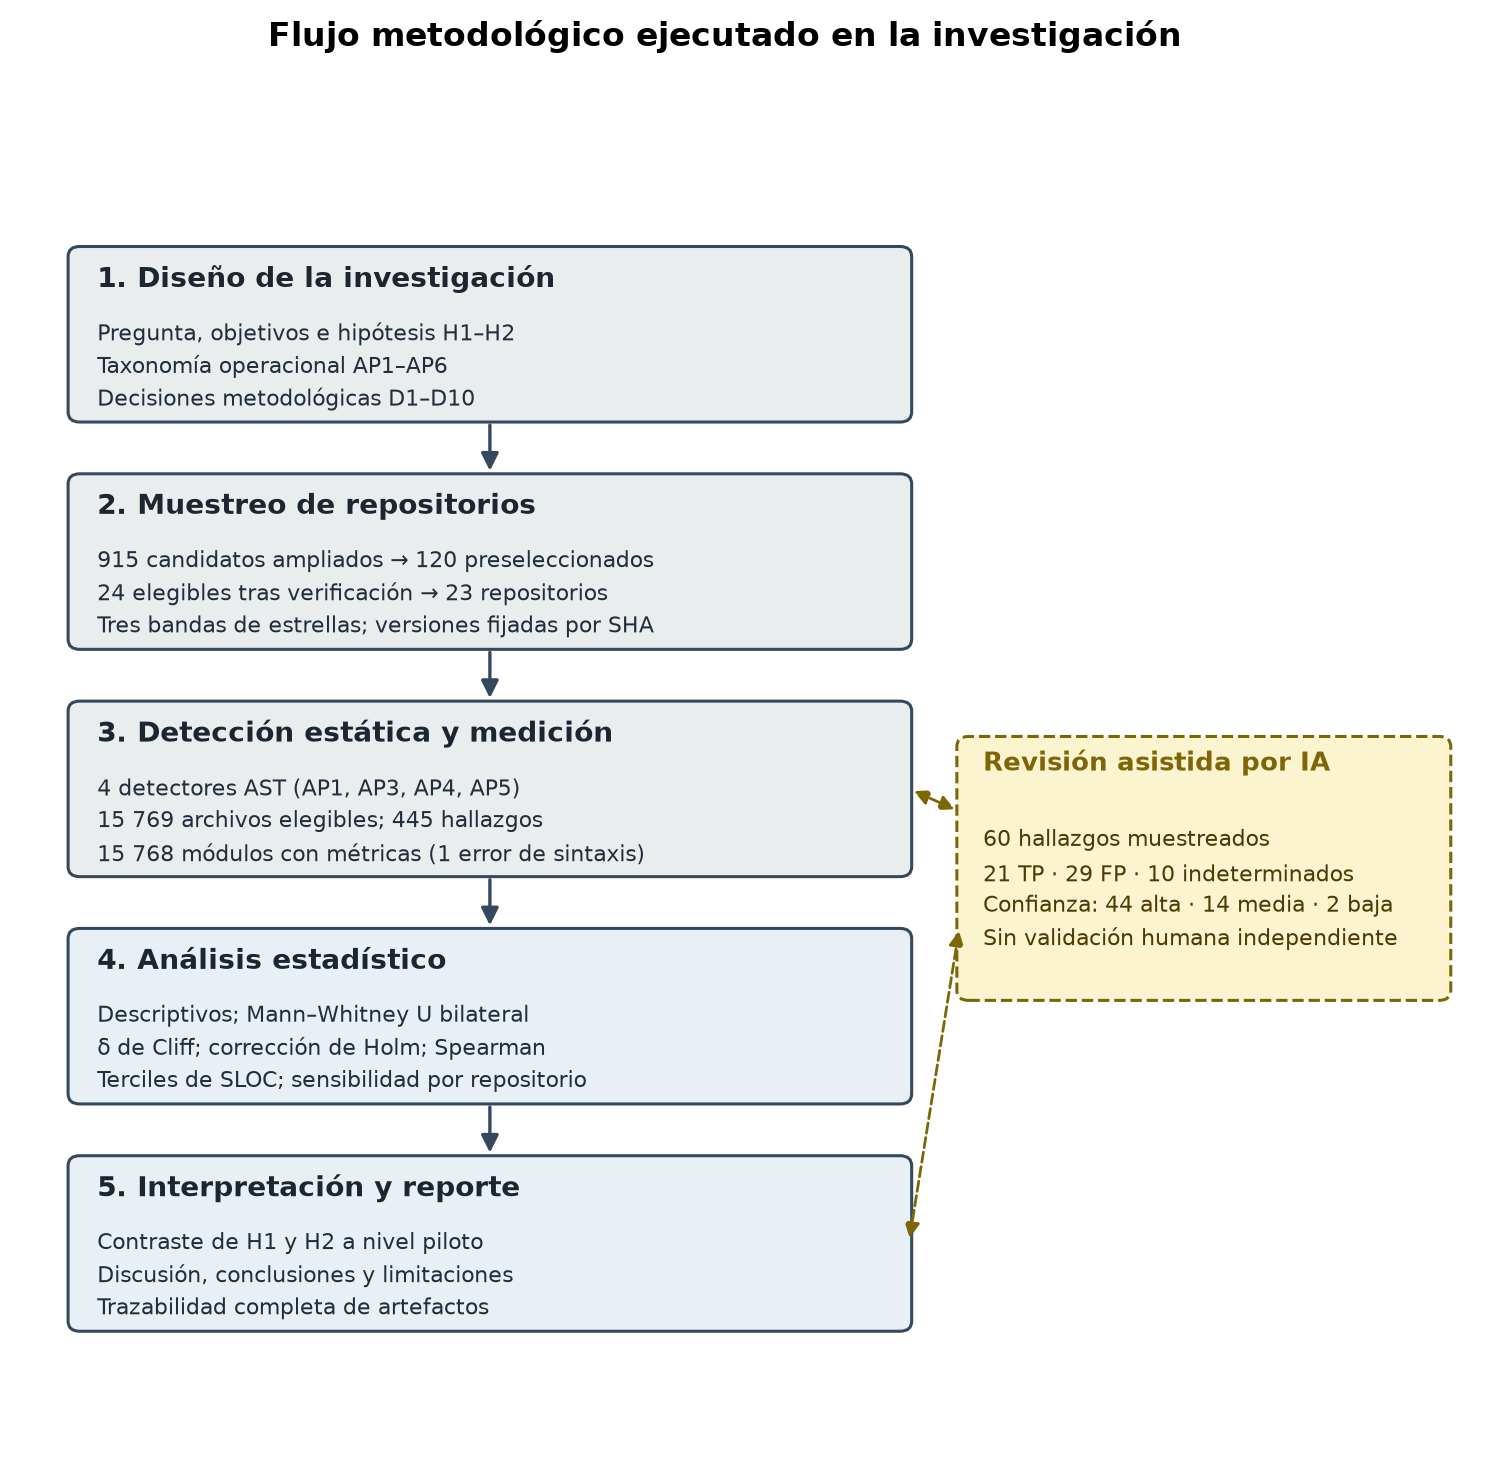
\includegraphics[width=\columnwidth]{figuras/fig01_flujo_metodologico.png}
\caption{Flujo metodológico ejecutado. La revisión asistida por IA se realizó en paralelo y no sustituye la validación humana independiente.}
\label{fig:flujo}
\end{figure}

El instrumento se implementó en Python y se organizó como un conjunto de scripts reproducibles. La detección utiliza la biblioteca estándar \texttt{ast}; el cálculo de complejidad e índice de mantenibilidad utiliza Radon; la manipulación tabular y el análisis estadístico utilizan pandas y SciPy; las figuras se generan con Matplotlib. Los scripts, los archivos de configuración y las salidas se conservan en el repositorio del proyecto, de modo que cualquier lector pueda repetir la secuencia desde los datos crudos hasta las tablas y figuras del informe.

\subsection{Población y muestra}

La población objetivo está constituida por aplicaciones de código abierto implementadas en Python que integran un modelo generativo de lenguaje y algún mecanismo de recuperación de información, y que además son públicamente accesibles en GitHub. No se incluyen aplicaciones propietarias, sistemas internos de organizaciones ni proyectos cuyo código no esté disponible. La muestra es no probabilística e intencional, estratificada por bandas de popularidad, y debe interpretarse como un piloto de conveniencia y no como una muestra representativa del universo de aplicaciones GenAI/RAG.

El universo de candidatos se construyó mediante consultas a la API de búsqueda de GitHub sobre tópicos asociados al dominio (por ejemplo, \texttt{rag}, \texttt{retrieval-augmented-generation}, \texttt{langchain}, \texttt{llamaindex} y \texttt{chatbot}), restringidas a Python, excluyendo forks y repositorios archivados, exigiendo actividad posterior al 23 de noviembre de 2025 y aplicando tres bandas de estrellas: 11--100, 101--1000 y más de 1000. Las consultas registradas arrojaron conteos que, tras deduplicación por nombre completo, dieron lugar a un universo histórico de 915 candidatos. Los intentos posteriores de ampliación mediante consultas agrupadas por tecnologías no produjeron resultados utilizables antes del límite de la API; en consecuencia, se conservó el universo histórico y se amplió el cribado a 120 filas estratificadas, cuarenta por banda. Esta decisión se documenta de forma transparente porque condiciona la composición de la muestra y porque impide afirmar que el universo se haya agotado.

La preselección aplicó un ordenamiento determinista por estrellas y excluyó, mediante palabras clave, repositorios cuya denominación o descripción sugería tutoriales, cursos, talleres, listas de recursos, ejemplos, demostraciones, libros de recetas, cuadernos o plantillas. Sobre las 120 filas preseleccionadas se verificaron, mediante llamadas autenticadas y seriales a la API, tres condiciones: existencia de un manifiesto raíz, presencia de tecnologías asociadas a RAG en los manifiestos y al menos veinte commits en el período de actividad. El resultado automatizado fue de 24 repositorios elegibles; 96 quedaron excluidos, principalmente por ausencia de tecnología RAG en los manifiestos, ausencia de manifiesto raíz o actividad insuficiente.

Los 24 repositorios elegibles se clonaron y se sometieron a una verificación local de relevancia que examinó el README y el código fuente en busca de evidencia conjunta de integración de LLM y de recuperación. Uno de ellos, \texttt{Tejas-TA/predikit}, no presentó evidencia conjunta suficiente y fue excluido, con lo que la muestra final quedó conformada por 23 repositorios. La composición por bandas fue de 13 repositorios con más de 1000 estrellas, 3 en la banda 101--1000 y 7 en la banda 11--100. La Tabla~\ref{tab:muestra} presenta la composición detallada y la Figura~\ref{fig:composicion} ilustra el embudo de selección y la distribución por popularidad.

El marco espacial del anteproyecto mencionó, a modo ilustrativo, proyectos como Quivr, Dify, RAGFlow y PrivateGPT. La muestra finalmente analizada no coincide con esa enumeración: el protocolo de cribado produjo un conjunto distinto, y este informe lo reporta tal como se ejecutó, sin sustituir los criterios operacionales por los nombres ilustrativos del diseño inicial.

\subsection{Operacionalización de variables}

La variable independiente principal es la presencia de al menos un antipatrón detectado en el módulo, codificada como variable binaria \texttt{con\_ap}. Como variable independiente secundaria se utiliza el número de hallazgos por módulo, \texttt{n\_ap}, que permite examinar si la asociación aumenta con la acumulación de hallazgos. Esta variable presenta una distribución fuertemente sesgada a cero: 15\,567 módulos no tienen hallazgos y solo 201 tienen uno o más.

Las variables dependientes primarias son tres. La complejidad ciclomática máxima del módulo, \texttt{cc\_max}, corresponde al mayor valor de complejidad ciclomática entre los bloques identificados por Radon; valores altos indican una estructura de control más ramificada. El índice de mantenibilidad, \texttt{mi}, es una métrica compuesta entre 0 y 100 en la que valores más altos indican mejor mantenibilidad. El acoplamiento aproximado a nivel de módulo, \texttt{cbo\_mod}, cuenta los módulos distintos importados que no pertenecen a la biblioteca estándar, incluyendo importaciones relativas documentadas. Es importante subrayar que \texttt{cbo\_mod} no es el CBO original de Chidamber y Kemerer \cite{chidamber_metrics_1994}: este último se define a nivel de clase y considera relaciones de diversa naturaleza, mientras que la aproximación utilizada se limita a dependencias de importación a nivel de archivo. Las variables secundarias son la complejidad ciclomática media, \texttt{cc\_media}, y las líneas de código fuente, \texttt{sloc}. La Tabla~\ref{tab:descriptivos} reporta la estadística descriptiva de las cinco métricas.

\subsection{Instrumento: taxonomía y detectores}

La taxonomía operacional se presenta en la Tabla~\ref{tab:taxonomia}. Comprende seis antipatrones, de los cuales cuatro fueron implementados y dos quedaron como ampliaciones no evaluadas. AP1, \emph{Hardcoded Prompt Infiltration}, detecta prompts extensos incrustados en funciones que concentran lógica de control. AP3, \emph{Hardcoded Provider Lock-in}, detecta la fijación literal de un proveedor o modelo en el constructor de un cliente de LLM. AP4, \emph{Monolithic RAG Function}, detecta funciones de más de sesenta líneas que combinan una llamada de recuperación y una llamada de generación. AP5, \emph{Non-Deterministic Exception Suppression}, detecta el silenciamiento de errores críticos mediante manejadores amplios que no vuelven a lanzar la excepción. AP2, \emph{Vector Store Leakage}, y AP6, \emph{Unvalidated Generation Output}, fueron definidos conceptualmente pero no implementados; por tanto, no fueron evaluados y su ausencia en los resultados no debe interpretarse como ausencia empírica.

\begin{table*}[t]
\centering
\scriptsize
\setlength{\tabcolsep}{3.5pt}
\caption{Taxonomía operacional de antipatrones y estado de implementación de los detectores}
\label{tab:taxonomia}
\begin{tabularx}{\textwidth}{@{}c >{\raggedright\arraybackslash}p{2.6cm} >{\raggedright\arraybackslash}X >{\raggedright\arraybackslash}p{2.2cm} >{\raggedright\arraybackslash}X l@{}}
\toprule
\textbf{ID} & \textbf{Nombre} & \textbf{Definición operacional} & \textbf{Atributo afectado} & \textbf{Regla de detección (AST)} & \textbf{Estado} \\
\midrule
\textbf{AP1} & Hardcoded Prompt Infiltration & Prompt extenso incrustado en una función que concentra lógica de control. & Mantenibilidad, evolvabilidad & Cadena o f-string $\geq$ 80 caracteres en función con control, vinculada a pista de prompt o llamada a LLM. & Implementado \\
\textbf{AP2} & Vector Store Leakage & Acceso vectorial desde la presentación o credencial literal. & Seguridad, separación de capas & Framework web con cliente vectorial, o credencial literal en el constructor. & No implementado \\
\textbf{AP3} & Hardcoded Provider Lock-in & Proveedor o modelo rígido sin abstracción configurable. & Portabilidad, mantenibilidad & Valor literal de \texttt{model} o \texttt{model\_name} reconocible en constructor o SDK documentado. & Implementado \\
\textbf{AP4} & Monolithic RAG Function & Una función concentra recuperación y generación. & Mantenibilidad, testabilidad & Función de más de 60 líneas con llamada de recuperación y llamada al LLM. & Implementado \\
\textbf{AP5} & Non-Deterministic Exception Suppression & Error crítico silenciado o convertido en fallback constante. & Confiabilidad & \texttt{try} con llamada crítica y manejador amplio sin \texttt{raise}; solo \texttt{pass}, registro o fallback constante. & Implementado \\
\textbf{AP6} & Unvalidated Generation Output & Salida generada llega a un sumidero sensible sin validación reconocible. & Confiabilidad, seguridad & Salida del LLM en \texttt{json.loads}, \texttt{eval}, \texttt{exec} o \texttt{.execute()} sin guardas. & No implementado \\
\bottomrule
\end{tabularx}
\end{table*}

Los detectores son reglas heurísticas sobre el AST y no análisis semántico ni de flujo de datos. Esta decisión reduce el costo computacional y permite escalar a miles de módulos, pero introduce un compromiso entre cobertura y precisión que la literatura sobre detección de olores arquitectónicos ha documentado ampliamente \cite{martini_identifying_2018,fontana_arcan_2017,mumtaz_systematic_2021}. Las reglas incorporan umbrales explícitos, vocabulario declarativo de proveedores, clases de LLM y llamadas de recuperación y generación, y exclusiones para reducir falsos positivos evidentes, como valores provenientes de configuración o entornos. Aun así, no pueden distinguir con certeza una construcción legítima de una práctica problemática, y esta limitación se retoma en la discusión y en el capítulo de limitaciones.

El escaneo excluye directorios y archivos que no representan código de producción: entornos virtuales, dependencias instaladas, builds, pruebas, documentación, ejemplos, migraciones, scripts auxiliares, archivos \texttt{conftest.py} y archivos cuyo nombre empieza por \texttt{test\_} o termina en \texttt{\_test.py}. También se excluyen archivos mayores de 1 MiB. Estos filtros buscan que la unidad observada sea el código que efectivamente forma parte de la aplicación, aunque la distinción entre código de producción y código auxiliar no siempre es nítida en proyectos pequeños.

\subsection{Extracción de métricas}

La extracción se ejecutó sobre exactamente los mismos módulos elegibles que recorrió el escáner, con el fin de mantener la correspondencia entre hallazgos y métricas. Para cada archivo se calculó el AST, se obtuvieron los bloques de complejidad con Radon, se calculó el índice de mantenibilidad y se contaron las líneas de código fuente y las raíces de importación no estándar. El proceso produjo 15\,768 filas de métricas a partir de 15\,769 archivos escaneados. La diferencia de una unidad se explica por un archivo de \texttt{BerriAI/litellm}, \texttt{litellm/secret\_managers/base\_secret\_manager.py}, que no pudo procesarse en la extracción de métricas por un error de sintaxis en la línea 9. El error se conserva en \texttt{metricas\_errors.csv} y no se corrigió ni se imputó.

La integridad de la unión entre hallazgos y métricas se verificó explícitamente: no hay hallazgos sin módulo de métricas asociado, no hay claves duplicadas y no hay valores faltantes en las cinco métricas. Estas comprobaciones son relevantes porque cualquier desalineación entre el archivo y la ruta relativa habría alterado la comparación entre grupos.

\subsection{Tratamiento estadístico}

El contraste primario utiliza la prueba U de Mann--Whitney bilateral para comparar los módulos con al menos un antipatrón frente a los módulos sin antipatrones, en cada una de las tres métricas primarias. Se eligió una prueba no paramétrica porque las distribuciones de las métricas son asimétricas, contienen valores extremos y no cumplen de forma plausible el supuesto de normalidad. La significancia se evaluó con un nivel $\alpha=0{,}05$ y se aplicó la corrección de Holm dentro de la familia de tres métricas primarias. Además del valor $p$, se reporta el $\delta$ de Cliff como tamaño de efecto, con la convención habitual de umbrales 0,147, 0,33 y 0,474 para efectos pequeño, mediano y grande, respectivamente. La dirección esperada se fijó antes del contraste: \texttt{cc\_max} y \texttt{cbo\_mod} mayores en el grupo con antipatrones, y \texttt{mi} menor en ese grupo.

La asociación entre el número de hallazgos por módulo y cada métrica se evaluó mediante el coeficiente de correlación de Spearman, nuevamente con corrección de Holm dentro de la familia de tres métricas. Se eligió Spearman porque \texttt{n\_ap} es un conteo con alta concentración en cero y porque la relación esperada no es necesariamente lineal. El coeficiente se interpreta como una medida de asociación monótona y no como una medida de efecto causal.

Para explorar la posible confusión por tamaño del código se construyeron terciles de \texttt{sloc} sobre el total de módulos. Los puntos de corte resultantes fueron 43 y 164 líneas, con un tercil inferior de hasta 43 líneas, un tercil medio entre 43 y 164 y un tercil superior por encima de 164. Dentro de cada tercil se repitió el contraste de Mann--Whitney para las tres métricas primarias. Estos nueve contrastes son exploratorios: no se corrigieron por multiplicidad y se reportan como evidencia parcial, no como confirmación. El tercil inferior contiene un solo módulo con antipatrón, de modo que su comparación inferencial no es fiable y se marca como \emph{n insuficiente}.

La sensibilidad por repositorio se evaluó agregando las métricas mediante la mediana de cada repositorio y comparando los repositorios con y sin hallazgos. El análisis es inconcluso por construcción: 2
\section{Cronograma y Presupuesto}\label{sec:cronograma}

\subsection{Cronograma}

El anteproyecto estimó un período de ejecución de aproximadamente diez semanas a partir de la aprobación, durante las cuales se desarrollarían la construcción y validación de la taxonomía, la selección de repositorios, la implementación del analizador estático, la extracción de métricas y el análisis estadístico. Esa estimación describe la intención del diseño, pero no permite reconstruir un cronograma detallado actividad por actividad: los registros del proyecto no conservan fechas de inicio y fin para cada una de esas actividades, ni la fecha formal de aprobación que serviría de ancla.

Lo que sí puede documentarse con evidencia son las marcas temporales de la ejecución técnica. La extracción de metadatos de la muestra se registró el 23 de noviembre de 2026 a las 20:13:30 UTC. La verificación autenticada de los repositorios preseleccionados se registró el mismo día a las 21:10:48 UTC. El escaneo de los 23 repositorios se ejecutó entre las 21:56:40 y las 21:59:41 UTC, y las etapas posteriores de métricas, análisis estadístico y generación de tablas y figuras se ejecutaron a continuación. Estos registros permiten afirmar que la fase de recolección y análisis automatizado se completó en una ventana de aproximadamente dos horas, pero no permiten fechar el diseño, la revisión de literatura, la escritura ni la corrección del informe.

Por esa razón, este documento no incluye un diagrama de Gantt. Un Gantt exige fechas de inicio y fin por actividad, hitos y dependencias; construirlo con valores estimados o retrocedidos introduciría información que no está respaldada por los registros y contradiría el principio de integridad científica que orienta el informe. La omisión es deliberada y se declara como una limitación administrativa, no como un olvido. Si el programa académico exige el diagrama, este deberá elaborarse a partir de la bitácora real del investigador o de las actas de aprobación, que no forman parte de los artefactos disponibles.

\subsection{Presupuesto}

Tampoco existe un registro contable del proyecto. No hay facturas, cotizaciones, comprobantes de pago, contratos de personal ni asignaciones presupuestales que permitan reportar costos monetarios por rubro. Por tanto, no se presenta una tabla de presupuesto y no se atribuyen valores a horas de trabajo, equipos, licencias, servicios en la nube o desplazamientos. Hacerlo sería una invención.

Lo que puede describirse es el conjunto de recursos efectivamente utilizados, sin asignarles un valor monetario. El trabajo se apoyó en herramientas de código abierto y en infraestructura preexistente: Python y su ecosistema científico (pandas, SciPy, Matplotlib), Radon para métricas de código, la API pública de GitHub para la recolección y verificación, Git para el control de versiones y una distribución local de LaTeX (MiKTeX) para la compilación del documento. No se adquirieron licencias comerciales, no se contrató personal y no se utilizaron servicios de cómputo en la nube con costo registrado. El almacenamiento y el procesamiento se realizaron en el equipo del investigador.

En términos de esfuerzo, la ejecución técnica automatizada fue breve, pero estuvo precedida por el diseño de la taxonomía, la implementación y depuración de los detectores, la definición de las decisiones metodológicas y la revisión de la literatura, actividades cuya dedicación horaria no quedó registrada. El informe reconoce esa ausencia y no la sustituye por estimaciones. La consecuencia práctica es que el proyecto puede auditarse en cuanto a sus artefactos y resultados, pero no en cuanto a su costo o a su calendarización formal.

\section{Recolección y Ordenamiento de la Información}

\subsection{Fuentes de información}

La recolección combinó cuatro fuentes. La primera fue la API de GitHub, utilizada para identificar candidatos, recuperar metadatos de popularidad y actividad, verificar manifiestos y confirmar la existencia de commits recientes. La segunda fue el código fuente de los repositorios clonados, fijado a un commit específico, que constituye la evidencia primaria para la detección de antipatrones y el cálculo de métricas. La tercera fueron los documentos del proyecto: la taxonomía operacional, las decisiones metodológicas D1--D10, los protocolos de validación y los informes de ejecución. La cuarta fue la literatura científica y técnica sobre antipatrones arquitectónicos, deuda técnica en sistemas de aprendizaje automático, detección estática y arquitecturas RAG.

El período de observación se delimitó con una fecha de corte de un año antes de la extracción. Las consultas exigieron actividad posterior al 23 de noviembre de 2025, de modo que la muestra priorizara proyectos activos y no repositorios abandonados. La extracción de metadatos se realizó el 23 de noviembre de 2026. Esta ventana de doce meses es una decisión de diseño y no una propiedad de los datos: un repositorio activo en ese período pudo haber cambiado después, pero el análisis se realizó sobre la versión fijada por SHA.

\subsection{Universo y cribado}

El universo inicial se construyó con consultas por tópicos asociados a RAG, agentes, LLM y marcos de recuperación, restringidas a Python, sin forks ni repositorios archivados y con al menos once estrellas. Las consultas se distribuyeron en tres bandas de popularidad para evitar que la muestra quedara dominada por proyectos muy grandes. Tras la deduplicación por nombre completo, el universo histórico quedó en 915 candidatos. Los intentos de ampliación mediante consultas agrupadas por tecnologías no devolvieron resultados utilizables antes del límite de búsqueda de la API, por lo que se conservó ese universo y se decidió ampliar el cribado en lugar de ampliar la recolección.

La preselección tomó 120 filas, cuarenta por banda, ordenadas de forma determinista por estrellas y filtradas con palabras clave que excluyen tutoriales, cursos, talleres, listas de recursos, ejemplos, demostraciones, libros de recetas, cuadernos y plantillas. Esta etapa no pretendía decidir la elegibilidad, sino reducir el costo de la verificación. La verificación posterior se aplicó a las 120 filas y comprobó tres condiciones: manifiesto raíz, tecnología asociada a RAG en los manifiestos y al menos veinte commits en el período. El resultado fue de 24 repositorios elegibles y 96 excluidos. Las causas de exclusión se conservaron en un archivo específico y se agrupan en tres familias: ausencia de tecnología RAG en los manifiestos, ausencia de manifiesto raíz y actividad insuficiente en el período.

Los 24 elegibles se clonaron y se sometieron a una verificación local de relevancia. Esta verificación leyó el README y el código en busca de evidencia conjunta de integración de un LLM y de un mecanismo de recuperación, y comparó el SHA clonado con el SHA verificado. Veintitrés repositorios cumplieron; \texttt{Tejas-TA/predikit} fue excluido porque su evidencia no mostraba conjuntamente integración de LLM y recuperación. La muestra final quedó en 23 repositorios. El embudo completo se ilustra en la Figura~\ref{fig:composicion}: 915 candidatos, 120 preseleccionados, 24 elegibles y 23 analizados.

\begin{figure*}[t]
\centering
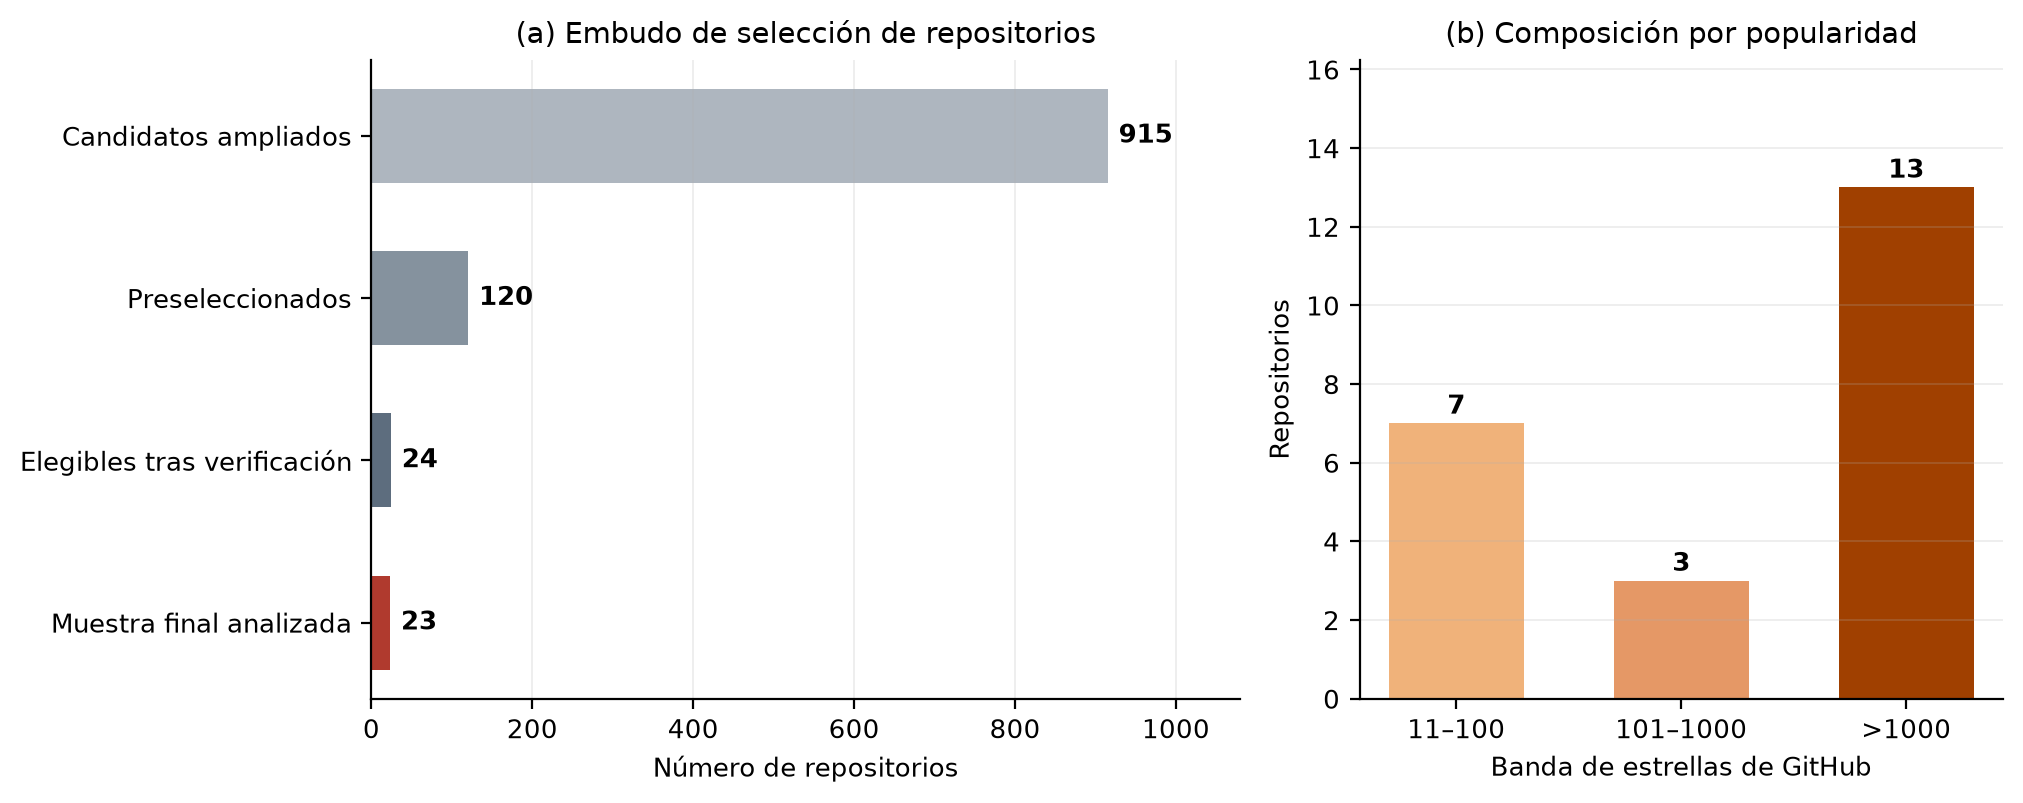
\includegraphics[width=0.92\textwidth]{figuras/fig02_composicion_muestra.png}
\caption{Composición de la muestra. (a) Embudo de selección desde los candidatos ampliados hasta la muestra final. (b) Distribución de los 23 repositorios por banda de estrellas.}
\label{fig:composicion}
\end{figure*}

\subsection{Composición de la muestra}

La Tabla~\ref{tab:muestra} presenta los 23 repositorios con su banda de popularidad, número de módulos elegibles, número de módulos con al menos un hallazgo, porcentaje de módulos afectados y número total de hallazgos. La muestra está desbalanceada por diseño: 13 repositorios pertenecen a la banda de más de 1000 estrellas, 3 a la banda 101--1000 y 7 a la banda 11--100. Este desbalance refleja tanto la disponibilidad de proyectos grandes y activos como el hecho de que la banda superior concentra más candidatos verificables. No se aplicó ponderación para corregirlo, de modo que los resultados describen la muestra tal como quedó constituida y no una población estratificada.

\begin{table*}[t]
\centering
\scriptsize
\setlength{\tabcolsep}{4pt}
\caption{Composición de la muestra: módulos y hallazgos por repositorio}
\label{tab:muestra}
\begin{tabularx}{\textwidth}{@{}X c r r r r@{}}
\toprule
\textbf{Repositorio} & \textbf{Banda} & \textbf{Módulos} & \textbf{Mód.\ con AP} & \textbf{\% con AP} & \textbf{Hallazgos} \\
\midrule
\texttt{multimindlab/multimind-sdk} & 11--100 & 392 & 42 & 10,71 & 194 \\
\texttt{bojieli/ai-agent-book} & >1000 & 1\,037 & 49 & 4,73 & 86 \\
\texttt{ai-bot-pro/achatbot} & 11--100 & 942 & 23 & 2,44 & 27 \\
\texttt{run-llama/llama\_index} & >1000 & 2\,114 & 13 & 0,61 & 21 \\
\texttt{headroomlabs-ai/headroom} & >1000 & 645 & 14 & 2,17 & 21 \\
\texttt{hoangsonww/Agentic-AI-Pipeline} & 11--100 & 73 & 2 & 2,74 & 15 \\
\texttt{onyx-dot-app/onyx} & >1000 & 2\,440 & 9 & 0,37 & 10 \\
\texttt{NJUxlj/Chinese-MedQA-Qwen2} & 11--100 & 137 & 6 & 4,38 & 10 \\
\texttt{arthurpanhku/DocSentinel} & 11--100 & 116 & 2 & 1,72 & 9 \\
\texttt{verygoodplugins/automem} & 101--1000 & 73 & 6 & 8,22 & 7 \\
\texttt{khoj-ai/khoj} & >1000 & 110 & 2 & 1,82 & 7 \\
\texttt{BerriAI/litellm} & >1000 & 3\,601 & 5 & 0,14 & 6 \\
\texttt{mlflow/mlflow} & >1000 & 1\,400 & 4 & 0,29 & 6 \\
\texttt{agentscope-ai/agentscope} & >1000 & 532 & 4 & 0,75 & 5 \\
\texttt{Mattral/filing-qa} & 11--100 & 70 & 5 & 7,14 & 5 \\
\texttt{1Panel-dev/MaxKB} & >1000 & 1\,010 & 5 & 0,50 & 5 \\
\texttt{HKUDS/LightRAG} & >1000 & 204 & 3 & 1,47 & 4 \\
\texttt{Cygnux-Labs/Tracekit} & 101--1000 & 235 & 3 & 1,28 & 3 \\
\texttt{ScrapeGraphAI/Scrapegraph-ai} & >1000 & 140 & 2 & 1,43 & 2 \\
\texttt{mem0ai/mem0} & >1000 & 257 & 1 & 0,39 & 1 \\
\texttt{getzep/graphiti} & >1000 & 210 & 1 & 0,48 & 1 \\
\texttt{ZhishaBai-web/help-you-find-job} & 11--100 & 8 & 0 & 0,00 & 0 \\
\texttt{LibreChat-AI/rag-api} & 101--1000 & 22 & 0 & 0,00 & 0 \\
\midrule
\textbf{Total} & --- & 15\,768 & 201 & 1,27 & 445 \\
\bottomrule
\end{tabularx}
\end{table*}

El tamaño de los repositorios es muy heterogéneo. \texttt{BerriAI/litellm} aporta 3601 módulos, \texttt{onyx-dot-app/onyx} 2440 y \texttt{run-llama/llama\_index} 2114, mientras que \texttt{ZhishaBai-web/help-you-find-job} aporta 8 y \texttt{LibreChat-AI/rag-api} 22. Esta heterogeneidad implica que las comparaciones a nivel de módulo están dominadas por unos pocos repositorios grandes y que los repositorios pequeños tienen poca influencia en los contrastes globales. La concentración de hallazgos agrava el problema: \texttt{multimindlab/multimind-sdk} aporta 194 hallazgos (43,6\,\%) y \texttt{bojieli/ai-agent-book} aporta 86 (19,3\,\%); juntos suman 280 de 445 hallazgos (62,9\,\%). La interpretación de los resultados debe tener presente esta concentración.

\subsection{Adquisición y fijación de versiones}

Cada repositorio se clonó en un directorio local y se verificó que el SHA de HEAD coincidiera con el SHA registrado en la selección. No hubo fallos de clonación en la muestra final. La fijación por SHA cumple dos funciones: hace reproducible el análisis y evita que una actualización del repositorio altere los resultados entre ejecuciones. El SHA de cada repositorio se conserva en \texttt{repos\_seleccionados.csv} y en el resumen de escaneo, de modo que un lector puede recuperar exactamente la versión analizada.

\subsection{Detección y extracción}

El escáner recorrió los 23 repositorios y procesó 15\,769 archivos Python elegibles. No se registraron errores de análisis sintáctico en el escaneo. Se emitieron 445 hallazgos, distribuidos en 201 módulos y 21 repositorios. La extracción de métricas se ejecutó sobre el mismo conjunto de archivos y produjo 15\,768 filas válidas; la única exclusión fue el archivo de \texttt{BerriAI/litellm} con error de sintaxis en la línea 9. La diferencia entre 15\,769 archivos escaneados y 15\,768 módulos con métricas es, por tanto, de una unidad y está documentada.

La Figura~\ref{fig:distribucion} resume dos dimensiones del resultado. El panel (a) muestra la distribución de los 445 hallazgos entre los cuatro antipatrones implementados: AP1 concentra 273 (61,35\,\%), AP5 152 (34,16\,\%), AP3 17 (3,82\,\%) y AP4 3 (0,67\,\%). El panel (b) muestra la cobertura a nivel de módulo en escala logarítmica: 201 módulos con al menos un hallazgo (1,27\,\%) frente a 15\,567 sin hallazgos (98,73\,\%). La escala logarítmica es necesaria porque la diferencia entre ambos grupos es de casi dos órdenes de magnitud; sin ella, el grupo con hallazgos sería prácticamente invisible.

\begin{figure*}[t]
\centering
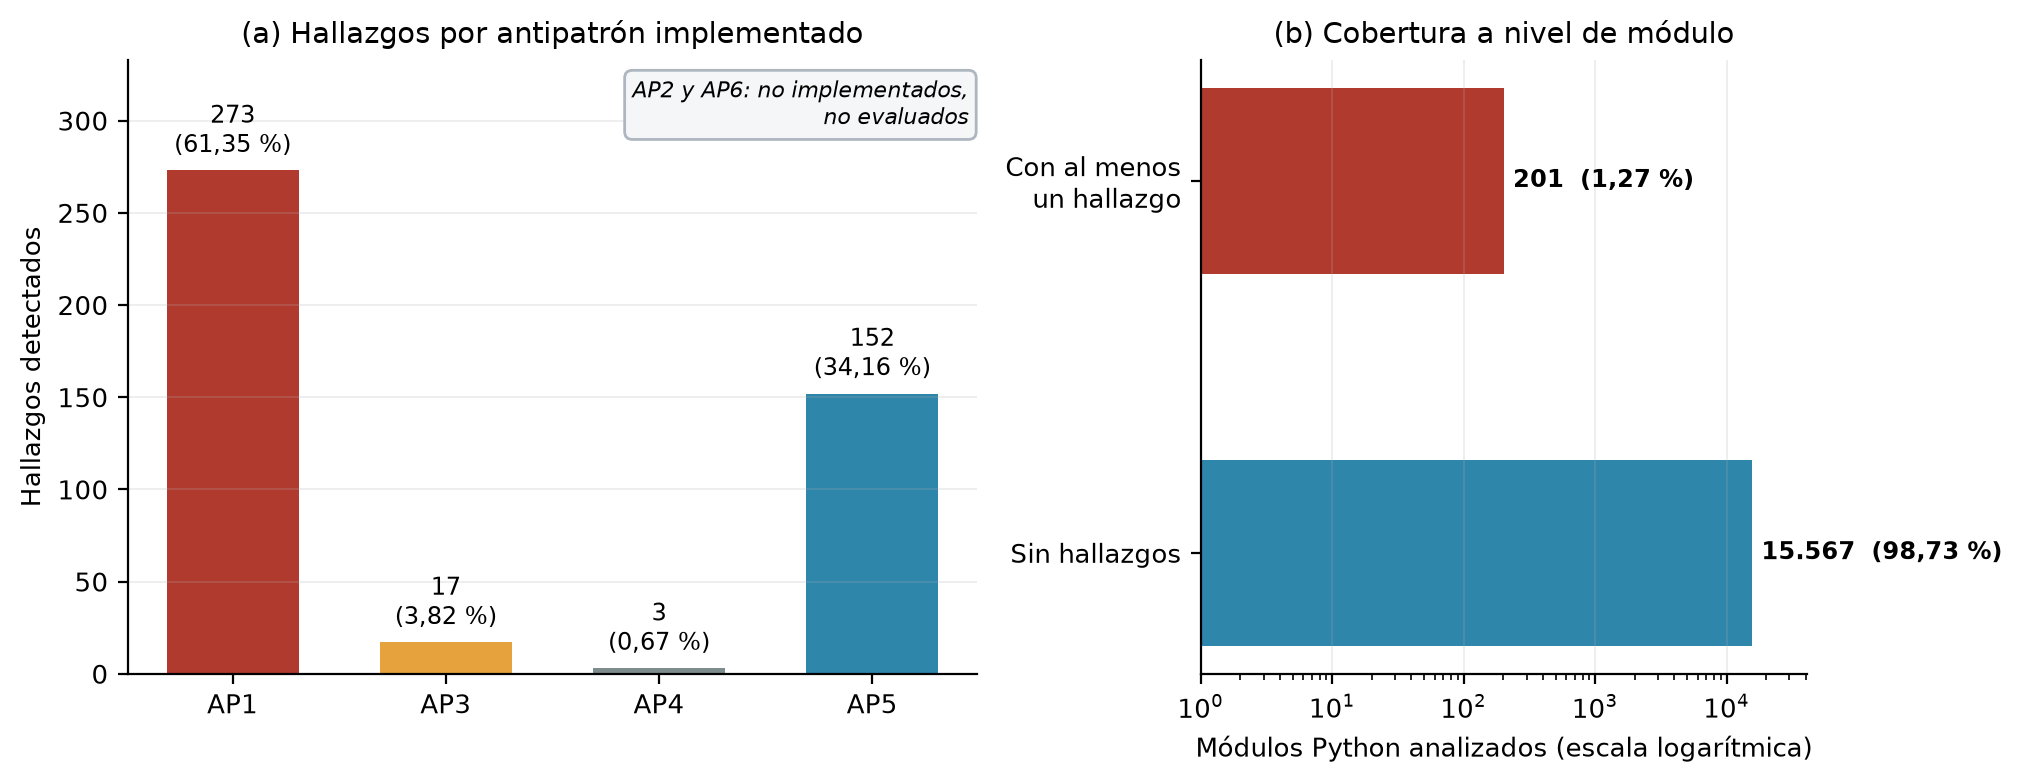
\includegraphics[width=0.92\textwidth]{figuras/fig03_distribucion_hallazgos.png}
\caption{Distribución de los hallazgos. (a) Hallazgos por antipatrón implementado; AP2 y AP6 no fueron implementados y no se evaluaron. (b) Módulos con y sin al menos un hallazgo, en escala logarítmica.}
\label{fig:distribucion}
\end{figure*}

\subsection{Organización y tabulación}

La información se organizó en archivos con granularidad explícita. El nivel de repositorio se conserva en \texttt{repos\_seleccionados.csv} y en \texttt{resumen\_repositorio.csv}; el nivel de módulo, en \texttt{metricas.csv}; el nivel de hallazgo, en \texttt{findings.csv}; y el nivel de análisis, en \texttt{estadisticas.csv}, \texttt{spearman.csv}, \texttt{resumen\_descriptivo.csv} y \texttt{decisiones\_hipotesis.csv}. La clave de unión entre hallazgos y métricas es la pareja \texttt{(repo, file)}, con rutas relativas a la raíz del repositorio. La matriz repositorio por antipatrón se conserva en \texttt{tabla\_repo\_ap.csv}, y la revisión asistida por IA en \texttt{validacion\_investigador.csv}.

La tabulación siguió tres reglas. Primero, no se agregaron filas ni se imputaron valores: los conteos de hallazgos, módulos y repositorios se derivan directamente de los archivos. Segundo, las métricas se calcularon una sola vez por módulo y se reutilizaron en todos los análisis. Tercero, las decisiones estadísticas se registraron en un archivo separado con sus criterios, entradas, resultado y limitaciones, de modo que la conclusión no dependiera de una interpretación posterior. La auditoría de consistencia verificó que no hay hallazgos sin métricas, que no hay claves duplicadas y que no hay valores faltantes en las métricas primarias.

\subsection{Presentación de los resultados}

El orden de presentación sigue la lógica del análisis. Primero se describe el volumen y la composición de la muestra. Luego se presenta la distribución de los antipatrones y su concentración por repositorio. A continuación se reportan los descriptivos de las métricas y el contraste primario entre grupos. Después se presentan las correlaciones, el análisis por terciles de tamaño y la sensibilidad por repositorio. Finalmente se reporta la revisión asistida por IA con su alcance limitado. Esta secuencia permite que el lector reconstruya el razonamiento antes de llegar a la discusión y a las conclusiones, y evita que los resultados se presenten como una colección de valores sin relación con las preguntas de investigación.
\section{Presentación de los Resultados}

\subsection{Distribución de los antipatrones detectados}

Los 445 hallazgos se distribuyen de forma marcadamente desigual entre los cuatro antipatrones implementados. La Tabla~\ref{tab:distribucion} muestra que AP1, \emph{Hardcoded Prompt Infiltration}, concentra 273 hallazgos (61,35\,\%) en 20 repositorios; AP5, \emph{Non-Deterministic Exception Suppression}, concentra 152 (34,16\,\%) en 14 repositorios; AP3, \emph{Hardcoded Provider Lock-in}, registra 17 (3,82\,\%) en 6 repositorios; y AP4, \emph{Monolithic RAG Function}, registra 3 (0,67\,\%) en 3 repositorios. AP2 y AP6 no aparecen en la tabla porque no fueron implementados: no se evaluaron y no debe interpretarse su ausencia como prevalencia cero.

\begin{table}[t]
\centering
\scriptsize
\setlength{\tabcolsep}{3pt}
\caption{Distribución de los hallazgos detectados por antipatrón}
\label{tab:distribucion}
\begin{tabularx}{\columnwidth}{@{}l >{\raggedright\arraybackslash}X r r r l@{}}
\toprule
\textbf{ID} & \textbf{Antipatrón} & \textbf{Hall.} & \textbf{\%} & \textbf{Rep.} & \textbf{Estado} \\
\midrule
\textbf{AP1} & Hardcoded Prompt Infiltration & 273 & 61,35 & 20 & Impl. \\
\textbf{AP2} & Vector Store Leakage & --- & --- & --- & No eval. \\
\textbf{AP3} & Hardcoded Provider Lock-in & 17 & 3,82 & 6 & Impl. \\
\textbf{AP4} & Monolithic RAG Function & 3 & 0,67 & 3 & Impl. \\
\textbf{AP5} & Non-Deterministic Exception Suppression & 152 & 34,16 & 14 & Impl. \\
\textbf{AP6} & Unvalidated Generation Output & --- & --- & --- & No eval. \\
\midrule
\textbf{Total} & & 445 & 100,00 & 21 & 4 de 6 \\
\bottomrule
\end{tabularx}
\end{table}

La diferencia entre AP1 y AP4 es de dos órdenes de magnitud. Esta diferencia puede reflejar tanto una presencia real desigual de los fenómenos como una sensibilidad distinta de las reglas. AP1 se activa con una condición relativamente común en aplicaciones que incorporan prompts en el código; AP4 exige una función de más de sesenta líneas que combine recuperación y generación, una construcción menos frecuente y más fácil de fragmentar en funciones auxiliares. La distribución observada no permite separar ambos factores, y por ello el informe no compara la prevalencia relativa de los antipatrones como si midiera una única propiedad del dominio.

\subsection{Hallazgos por repositorio y concentración}

La Figura~\ref{fig:repositorios} ordena los 23 repositorios por número total de hallazgos y descompone cada barra por antipatrón. Dos repositorios dominan la distribución: \texttt{multimindlab/multimind-sdk} con 194 hallazgos y \texttt{bojieli/ai-agent-book} con 86. Juntos representan 280 de 445 hallazgos (62,9\,\%). Les siguen \texttt{ai-bot-pro/achatbot} con 27, \texttt{headroomlabs-ai/headroom} y \texttt{run-llama/llama\_index} con 21 cada uno, y \texttt{hoangsonww/Agentic-AI-Pipeline} con 15. En el extremo opuesto, 21 repositorios tienen al menos un hallazgo, mientras que \texttt{ZhishaBai-web/help-you-find-job} (8 módulos) y \texttt{LibreChat-AI/rag-api} (22 módulos) no registran ninguno.

\begin{figure*}[t]
\centering
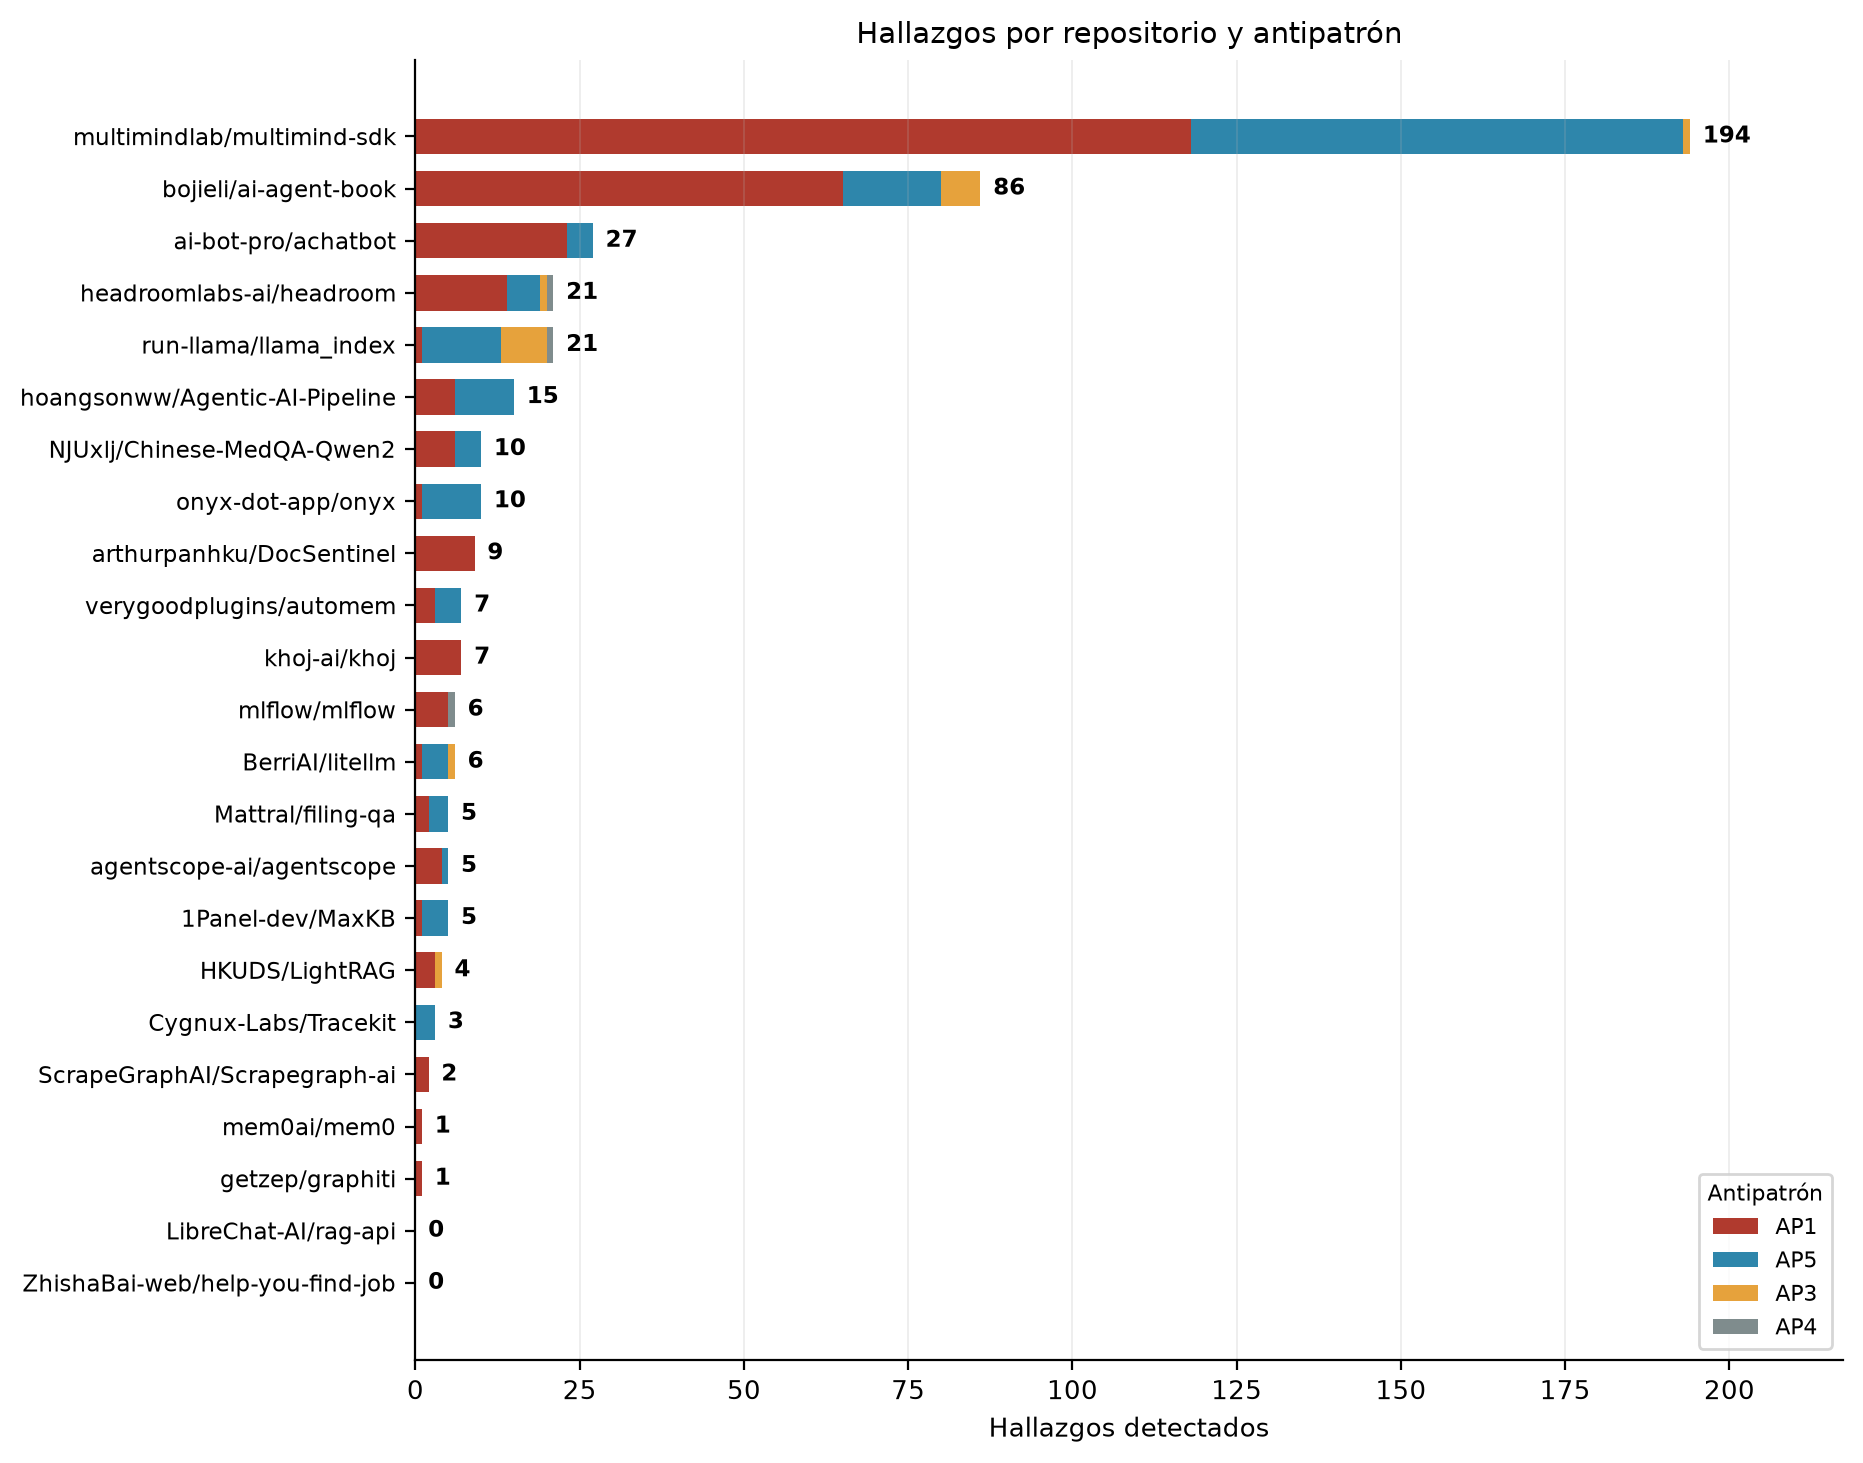
\includegraphics[width=0.90\textwidth]{figuras/fig04_hallazgos_por_repositorio.png}
\caption{Hallazgos por repositorio y antipatrón. Los repositorios se ordenan por número total de hallazgos. Los dos repositorios sin hallazgos aparecen al final con valor cero.}
\label{fig:repositorios}
\end{figure*}

La concentración tiene dos consecuencias. Primero, los contrastes globales están influidos por unos pocos repositorios: si \texttt{multimindlab/multimind-sdk} se comporta de forma atípica, su peso en el total puede arrastrar las comparaciones. Segundo, la unidad de observación independiente no es el módulo sino, en el mejor de los casos, el repositorio, y con solo dos repositorios sin hallazgos no es posible una comparación agregada estable. El análisis de sensibilidad por repositorio, presentado más adelante, confirma esta dificultad.

También es relevante que el repositorio con más hallazgos no sea el más grande. \texttt{multimindlab/multimind-sdk} tiene 392 módulos, frente a 3601 de \texttt{BerriAI/litellm} o 2440 de \texttt{onyx-dot-app/onyx}. Su tasa de módulos con antipatrón es 10,71\,\%, la más alta de la muestra, mientras que la de \texttt{BerriAI/litellm} es 0,14\,\%. Esta diferencia sugiere que la densidad de antipatrones depende de prácticas de diseño y no solo del tamaño del repositorio, aunque el diseño transversal no permite atribuir la diferencia a una causa específica.

\subsection{Estadística descriptiva}

La Tabla~\ref{tab:descriptivos} reporta media, desviación estándar, mediana, cuartiles y extremos para las cinco métricas en los grupos \emph{todos}, \emph{con AP} y \emph{sin AP}. Las distribuciones son asimétricas y presentan valores extremos, de modo que la mediana es un resumen más informativo que la media. En \texttt{cc\_max}, la mediana pasa de 5 en el grupo sin antipatrones a 14 en el grupo con antipatrones; en \texttt{mi}, de 68,04 a 39,74; en \texttt{cbo\_mod}, de 2 a 3; y en \texttt{sloc}, de 87 a 399. Las medias siguen la misma dirección, pero son considerablemente mayores en el grupo con antipatrones, especialmente en \texttt{sloc} (614,05 frente a 204,04), lo que evidencia la cola de módulos grandes.

\begin{table*}[t]
\centering
\footnotesize
\setlength{\tabcolsep}{5pt}
\caption{Estadística descriptiva de las métricas por grupo}
\label{tab:descriptivos}
\begin{tabularx}{\textwidth}{@{}X l r r r r r r r r@{}}
\toprule
\textbf{Métrica} & \textbf{Grupo} & \textbf{n} & \textbf{Media} & \textbf{DE} & \textbf{Mediana} & \textbf{Q1} & \textbf{Q3} & \textbf{Mín.} & \textbf{Máx.} \\
\midrule
\texttt{cc\_max} & Todos & 15\,768 & 8,28 & 14,26 & 5,00 & 1,00 & 11,00 & 0,00 & 533,00 \\
\texttt{cc\_max} & Con AP & 201 & 22,35 & 28,48 & 14,00 & 9,00 & 24,00 & 1,00 & 227,00 \\
\texttt{cc\_max} & Sin AP & 15\,567 & 8,10 & 13,89 & 5,00 & 1,00 & 10,00 & 0,00 & 533,00 \\
\midrule
\texttt{mi} & Todos & 15\,768 & 68,47 & 27,20 & 67,57 & 49,09 & 100,00 & 0,00 & 100,00 \\
\texttt{mi} & Con AP & 201 & 38,09 & 20,32 & 39,74 & 25,71 & 51,79 & 0,00 & 100,00 \\
\texttt{mi} & Sin AP & 15\,567 & 68,87 & 27,06 & 68,04 & 49,46 & 100,00 & 0,00 & 100,00 \\
\midrule
\texttt{cbo\_mod} & Todos & 15\,768 & 2,20 & 2,06 & 2,00 & 1,00 & 3,00 & 0,00 & 43,00 \\
\texttt{cbo\_mod} & Con AP & 201 & 3,76 & 2,73 & 3,00 & 2,00 & 5,00 & 0,00 & 15,00 \\
\texttt{cbo\_mod} & Sin AP & 15\,567 & 2,18 & 2,04 & 2,00 & 1,00 & 3,00 & 0,00 & 43,00 \\
\midrule
\texttt{cc\_media} & Todos & 15\,768 & 2,95 & 3,06 & 2,43 & 1,00 & 4,01 & 0,00 & 120,00 \\
\texttt{cc\_media} & Con AP & 201 & 5,60 & 3,05 & 5,00 & 3,74 & 6,95 & 1,00 & 22,03 \\
\texttt{cc\_media} & Sin AP & 15\,567 & 2,92 & 3,04 & 2,38 & 1,00 & 4,00 & 0,00 & 120,00 \\
\midrule
\texttt{sloc} & Todos & 15\,768 & 209,27 & 478,66 & 89,00 & 26,00 & 224,00 & 0,00 & 13\,018,00 \\
\texttt{sloc} & Con AP & 201 & 614,05 & 983,40 & 399,00 & 209,00 & 660,00 & 21,00 & 10\,241,00 \\
\texttt{sloc} & Sin AP & 15\,567 & 204,04 & 466,38 & 87,00 & 25,00 & 219,00 & 0,00 & 13\,018,00 \\
\bottomrule
\end{tabularx}
\end{table*}

La comparación de medianas y medias revela el efecto de la asimetría. En \texttt{cc\_max}, la media del grupo con antipatrones (22,35) supera ampliamente su mediana (14), y su máximo alcanza 227; en \texttt{sloc}, la media (614,05) casi duplica la mediana (399) y el máximo llega a 10\,241. Estas diferencias justifican el uso de pruebas no paramétricas y de medidas de efecto basadas en rangos, y también advierten que una comparación de medias habría sobreestimado la separación entre grupos.

\subsection{Contraste primario}

La Tabla~\ref{tab:mann-whitney} presenta los tres contrastes primarios. Las tres métricas muestran diferencias estadísticamente significativas después de la corrección de Holm, con valores $p$ extremadamente pequeños y tamaños de efecto en la dirección esperada. En \texttt{cc\_max}, la mediana es 14 frente a 5, con $U=2\,517\,200{,}5$, $p_{Holm}=4{,}85\times10^{-50}$ y $\delta=+0{,}609$, un efecto grande. En \texttt{mi}, la mediana es 39,74 frente a 68,04, con $U=586\,956{,}5$, $p_{Holm}=2{,}00\times10^{-53}$ y $\delta=-0{,}625$, también un efecto grande. En \texttt{cbo\_mod}, la mediana es 3 frente a 2, con $U=2\,194\,635$, $p_{Holm}=7{,}41\times10^{-24}$ y $\delta=+0{,}403$, un efecto mediano.

\begin{table*}[t]
\centering
\footnotesize
\setlength{\tabcolsep}{4pt}
\caption{Contraste primario de Mann--Whitney U entre módulos con y sin antipatrones detectados}
\label{tab:mann-whitney}
\begin{tabularx}{\textwidth}{@{}X r r r r r l l r l@{}}
\toprule
\textbf{Métrica} & \textbf{n con} & \textbf{n sin} & \textbf{Med.\ con} & \textbf{Med.\ sin} & \textbf{U} & \textbf{p} & \textbf{p Holm} & \textbf{$\delta$} & \textbf{Magnitud} \\
\midrule
\texttt{cc\_max} & 201 & 15\,567 & 14,00 & 5,00 & 2\,517\,200,5 & $2{,}42 \times 10^{-50}$ & $4{,}85 \times 10^{-50}$ & $+0{,}609$ & Grande \\
\texttt{mi} & 201 & 15\,567 & 39,74 & 68,04 & 586\,956,5 & $6{,}68 \times 10^{-54}$ & $2{,}00 \times 10^{-53}$ & $-0{,}625$ & Grande \\
\texttt{cbo\_mod} & 201 & 15\,567 & 3,00 & 2,00 & 2\,194\,635,0 & $7{,}41 \times 10^{-24}$ & $7{,}41 \times 10^{-24}$ & $+0{,}403$ & Mediano \\
\bottomrule
\end{tabularx}
\end{table*}

La Figura~\ref{fig:metricas} ilustra las distribuciones mediante diagramas de caja. Los valores atípicos se omiten para facilitar la lectura, pero las medianas y los tamaños de efecto se conservan en la tabla. La separación visual es clara en las tres métricas: el grupo con antipatrones tiene cajas desplazadas hacia mayor complejidad, menor mantenibilidad y mayor acoplamiento. Sin embargo, la superposición entre grupos es considerable, especialmente en \texttt{cbo\_mod}, donde las cajas comparten buena parte de su rango. La existencia de una diferencia de grupo no implica que todos los módulos con antipatrón sean problemáticos ni que todos los módulos sin antipatrón estén sanos.

\begin{figure*}[t]
\centering
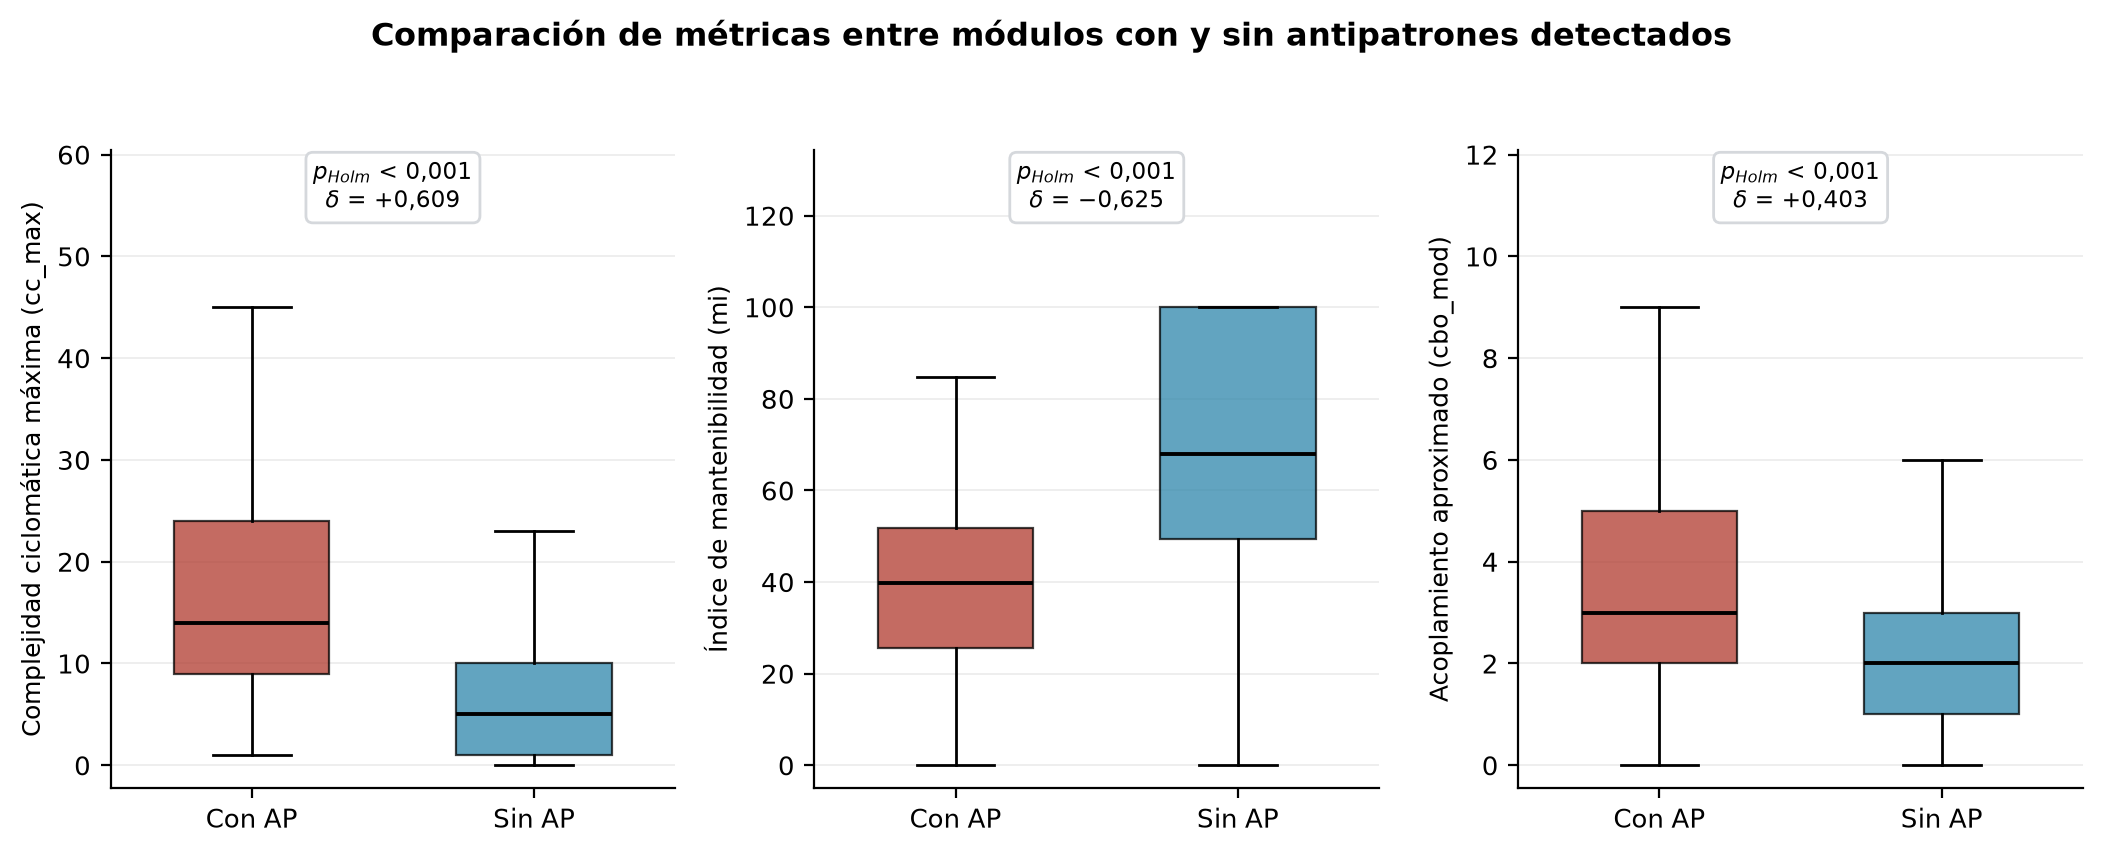
\includegraphics[width=0.95\textwidth]{figuras/fig05_comparacion_metricas.png}
\caption{Comparación de las tres métricas primarias entre módulos con y sin antipatrones detectados. Se omiten los valores atípicos para facilitar la lectura; las medianas y los tamaños de efecto se reportan en la Tabla~\ref{tab:mann-whitney}.}
\label{fig:metricas}
\end{figure*}

\subsection{Correlaciones de Spearman}

La Tabla~\ref{tab:spearman} presenta la asociación entre el número de hallazgos por módulo y las tres métricas primarias. Las tres correlaciones son estadísticamente significativas después de la corrección de Holm, pero de magnitud débil. \texttt{cc\_max} presenta $\rho=+0{,}119$ ($p_{Holm}=2{,}03\times10^{-50}$), \texttt{mi} presenta $\rho=-0{,}123$ ($p_{Holm}=6{,}78\times10^{-54}$) y \texttt{cbo\_mod} presenta $\rho=+0{,}080$ ($p_{Holm}=6{,}06\times10^{-24}$). Las direcciones coinciden con lo esperado: más hallazgos se asocian con mayor complejidad, menor mantenibilidad y mayor acoplamiento, pero la proporción de variación explicada es muy baja.

\begin{table*}[t]
\centering
\footnotesize
\setlength{\tabcolsep}{5pt}
\caption{Correlaciones de Spearman entre el número de hallazgos por módulo y las métricas}
\label{tab:spearman}
\begin{tabularx}{\textwidth}{@{}l r l l r >{\raggedright\arraybackslash}X@{}}
\toprule
\textbf{Métrica} & \textbf{$\rho$} & \textbf{p} & \textbf{p Holm} & \textbf{n} & \textbf{Lectura} \\
\midrule
\texttt{cc\_max} & $+0{,}119$ & $1{,}01 \times 10^{-50}$ & $2{,}03 \times 10^{-50}$ & 15\,768 & Asociación positiva débil \\
\texttt{mi} & $-0{,}123$ & $2{,}26 \times 10^{-54}$ & $6{,}78 \times 10^{-54}$ & 15\,768 & Asociación negativa débil \\
\texttt{cbo\_mod} & $+0{,}080$ & $6{,}06 \times 10^{-24}$ & $6{,}06 \times 10^{-24}$ & 15\,768 & Asociación positiva muy débil \\
\bottomrule
\end{tabularx}
\end{table*}

La Figura~\ref{fig:correlacion} muestra las distribuciones de cada métrica según el número de hallazgos por módulo, agrupado en cero, uno, dos, tres a cinco y seis o más. El grupo con cero hallazgos contiene 15\,567 módulos y domina la escala; los grupos con hallazgos son pequeños (129, 31, 23 y 18 módulos, respectivamente). Las medianas se desplazan en la dirección esperada, pero las cajas se superponen ampliamente y los grupos con más hallazgos no muestran una progresión monotónica perfecta. La correlación débil es consistente con esta imagen: hay una tendencia, no una relación estrecha.

\begin{figure*}[t]
\centering
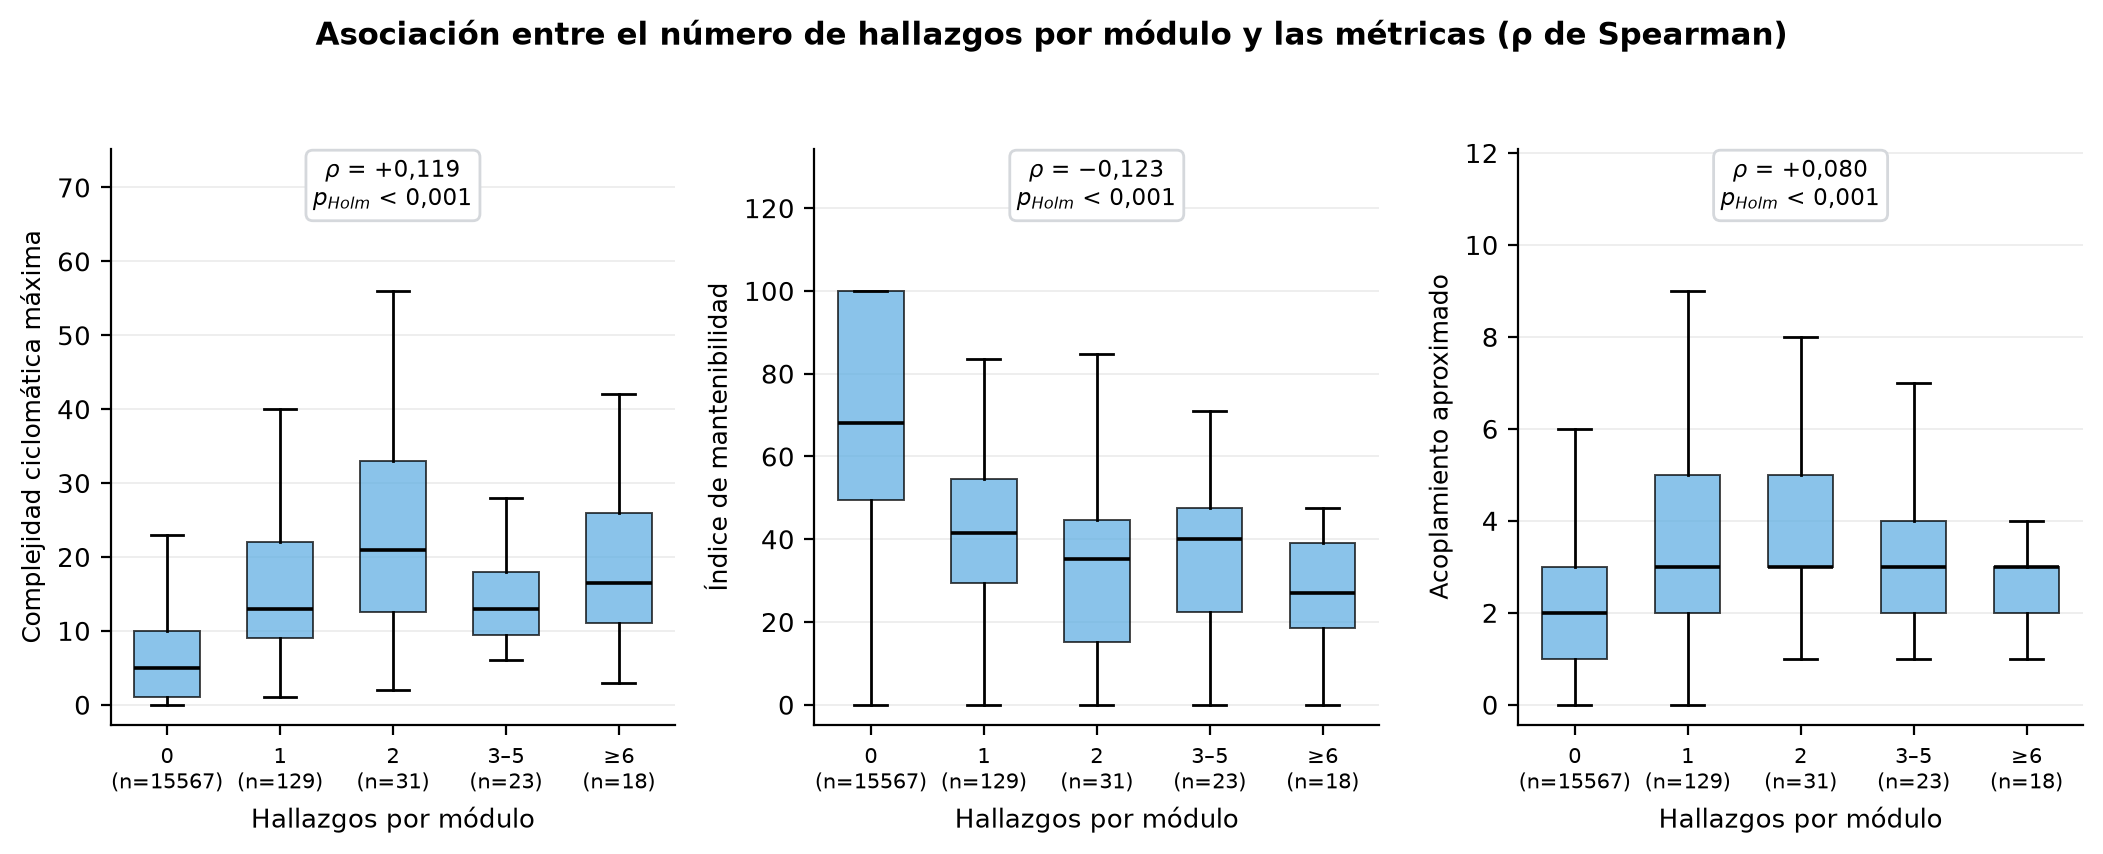
\includegraphics[width=0.95\textwidth]{figuras/fig06_correlacion_spearman.png}
\caption{Distribución de las métricas según el número de hallazgos por módulo. Los tamaños de grupo se indican en el eje horizontal; $\rho$ corresponde al coeficiente de Spearman sobre la variable de conteo completa.}
\label{fig:correlacion}
\end{figure*}

La diferencia entre el tamaño de efecto del contraste de grupos y la correlación merece atención. El $\delta$ de Cliff compara dos grupos y es grande para \texttt{cc\_max} y \texttt{mi}, mientras que $\rho$ es débil porque la mayoría de los módulos se concentra en cero y la variable de conteo tiene poca variación efectiva. Ambos resultados son compatibles: existe una separación entre \emph{tener} y \emph{no tener} antipatrones, pero el número de hallazgos por módulo no predice con precisión la magnitud de las métricas.

\subsection{Análisis por terciles de tamaño}

La Tabla~\ref{tab:terciles} y la Figura~\ref{fig:terciles} presentan el análisis exploratorio por terciles de \texttt{sloc}. El tercil inferior (hasta 43 líneas) contiene un solo módulo con antipatrón frente a 5313 sin antipatrón; por ello, sus valores se reportan pero no se interpretan inferencialmente y se marcan como \emph{n insuficiente}. El tercil medio (43--164 líneas) contiene 40 módulos con antipatrón y 5175 sin antipatrón; las tres métricas muestran diferencias significativas, con efecto mediano en \texttt{cc\_max} ($\delta=+0{,}391$) y efectos pequeños en \texttt{mi} ($\delta=-0{,}276$) y \texttt{cbo\_mod} ($\delta=+0{,}230$). El tercil superior (más de 164 líneas) contiene 160 módulos con antipatrón y 5079 sin antipatrón; \texttt{cc\_max} y \texttt{mi} mantienen efectos pequeños ($\delta=+0{,}270$ y $\delta=-0{,}306$), mientras que \texttt{cbo\_mod} presenta una diferencia estadísticamente significativa pero de efecto despreciable ($\delta=+0{,}142$), con medianas iguales a 3 en ambos grupos.

\begin{table*}[t]
\centering
\scriptsize
\setlength{\tabcolsep}{3.5pt}
\caption{Análisis exploratorio por terciles de líneas de código (SLOC)}
\label{tab:terciles}
\begin{tabularx}{\textwidth}{@{}l l l r r r r l r l >{\raggedright\arraybackslash}X@{}}
\toprule
\textbf{Tercil} & \textbf{SLOC} & \textbf{Métrica} & \textbf{n con} & \textbf{n sin} & \textbf{Med.\ con} & \textbf{Med.\ sin} & \textbf{p} & \textbf{$\delta$} & \textbf{Magnitud} & \textbf{Estado} \\
\midrule
Inferior & $\leq 43$ & \texttt{cc\_max} & 1 & 5\,313 & 1,00 & 1,00 & --- & $+0{,}184$ & Pequeño & \textit{n insuficiente} \\
 &  & \texttt{mi} & 1 & 5\,313 & 83,47 & 100,00 & --- & $-0{,}686$ & Grande & \textit{n insuficiente} \\
 &  & \texttt{cbo\_mod} & 1 & 5\,313 & 1,00 & 1,00 & --- & $+0{,}016$ & Despreciable & \textit{n insuficiente} \\
\midrule
Medio & 43--164 & \texttt{cc\_max} & 40 & 5\,175 & 8,50 & 5,00 & $1{,}87 \times 10^{-5}$ & $+0{,}391$ & Mediano & Significativo \\
 &  & \texttt{mi} & 40 & 5\,175 & 62,18 & 68,12 & 0,00257 & $-0{,}276$ & Pequeño & Significativo \\
 &  & \texttt{cbo\_mod} & 40 & 5\,175 & 2,00 & 2,00 & 0,00967 & $+0{,}230$ & Pequeño & Significativo \\
\midrule
Superior & $>164$ & \texttt{cc\_max} & 160 & 5\,079 & 15,50 & 12,00 & $5{,}46 \times 10^{-9}$ & $+0{,}270$ & Pequeño & Significativo \\
 &  & \texttt{mi} & 160 & 5\,079 & 35,09 & 43,69 & $4{,}17 \times 10^{-11}$ & $-0{,}306$ & Pequeño & Significativo \\
 &  & \texttt{cbo\_mod} & 160 & 5\,079 & 3,00 & 3,00 & 0,00186 & $+0{,}142$ & Despreciable & Significativo \\
\bottomrule
\end{tabularx}
\end{table*}

\begin{figure*}[t]
\centering
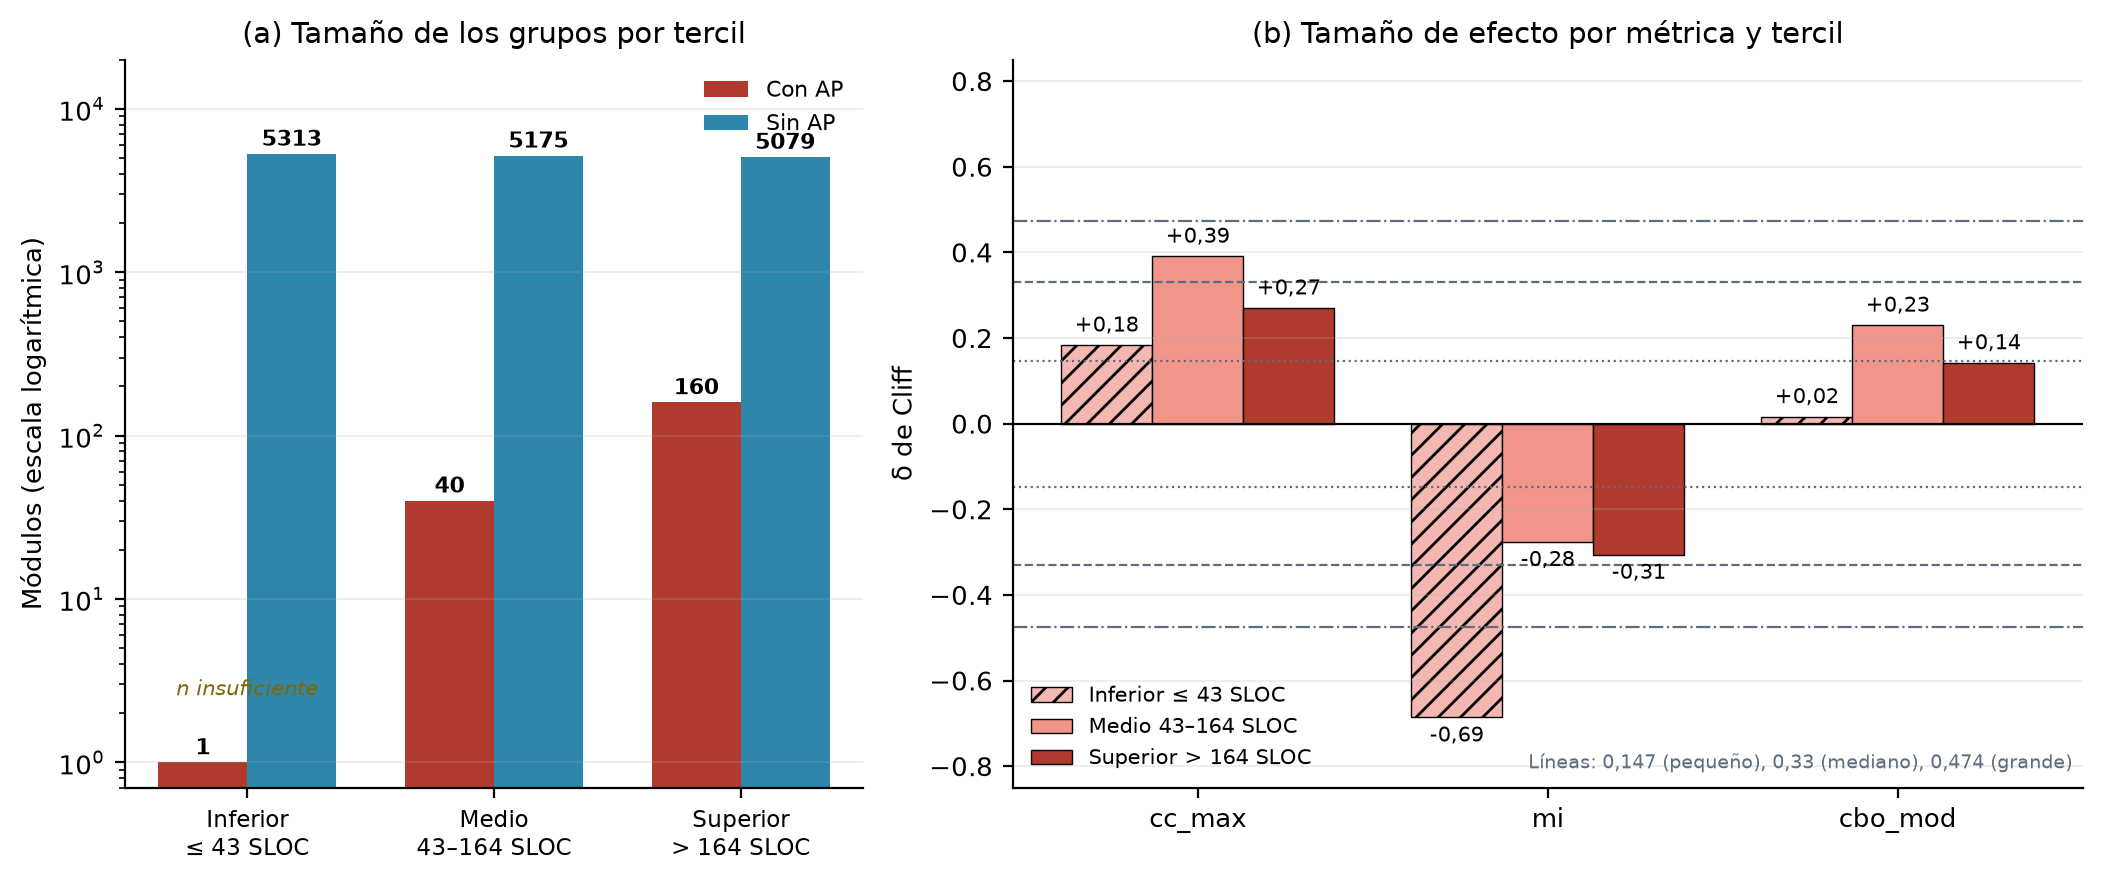
\includegraphics[width=0.92\textwidth]{figuras/fig07_terciles_sloc.png}
\caption{Análisis por terciles de líneas de código. (a) Tamaño de los grupos con y sin antipatrones en escala logarítmica. (b) Tamaño de efecto de Cliff por métrica y tercil; las barras rayadas corresponden al tercil inferior, con un solo módulo con antipatrón.}
\label{fig:terciles}
\end{figure*}

Estos resultados ofrecen evidencia parcial de que la asociación no se explica exclusivamente por el tamaño del código: dentro del tercil medio y del superior, las diferencias persisten en la dirección esperada para \texttt{cc\_max} y \texttt{mi}. Sin embargo, no la controlan por completo. El tercil superior sigue conteniendo módulos más grandes que el medio, y la estratificación por una sola variable no elimina la confusión residual por otras características del repositorio o del diseño. Además, los nueve contrastes por tercil son exploratorios y no fueron corregidos por multiplicidad; el valor $p=0{,}00186$ de \texttt{cbo\_mod} en el tercil superior debe leerse con cautela, sobre todo porque su tamaño de efecto es despreciable.

\subsection{Sensibilidad por repositorio}

La Tabla~\ref{tab:sensibilidad} presenta la comparación agregada de medianas por repositorio. Los 21 repositorios con hallazgos se comparan con los 2 repositorios sin hallazgos, un tamaño de grupo muy inferior al mínimo de cinco que el protocolo exige. Por esa razón, los tres contrastes se marcan como \emph{n insuficiente} y no se reportan valores $p$. Las diferencias descriptivas son mixtas: \texttt{cc\_max} es mayor en los repositorios con antipatrones (mediana 5 frente a 3,25; $\delta=+0{,}548$), lo que coincide con la dirección esperada; \texttt{mi} es ligeramente mayor en los repositorios con antipatrones (64,39 frente a 62,02; $\delta=+0{,}095$), en contra de lo esperado; y \texttt{cbo\_mod} es menor en los repositorios con antipatrones (2 frente a 2,25; $\delta=-0{,}452$), también en contra de lo esperado.

\begin{table*}[t]
\centering
\footnotesize
\setlength{\tabcolsep}{4pt}
\caption{Análisis de sensibilidad agregado por repositorio (medianas por repositorio)}
\label{tab:sensibilidad}
\begin{tabularx}{\textwidth}{@{}l r r r r r >{\raggedright\arraybackslash}X c l@{}}
\toprule
\textbf{Métrica} & \textbf{n con} & \textbf{n sin} & \textbf{Med.\ con} & \textbf{Med.\ sin} & \textbf{$\delta$} & \textbf{Dirección esperada} & \textbf{¿Coincide?} & \textbf{Estado} \\
\midrule
\texttt{cc\_max} & 21 & 2 & 5,00 & 3,25 & $+0{,}548$ & Mayor en con AP & Sí & \textit{n insuficiente} \\
\texttt{mi} & 21 & 2 & 64,39 & 62,02 & $+0{,}095$ & Menor en con AP & No & \textit{n insuficiente} \\
\texttt{cbo\_mod} & 21 & 2 & 2,00 & 2,25 & $-0{,}452$ & Mayor en con AP & No & \textit{n insuficiente} \\
\bottomrule
\end{tabularx}
\end{table*}

Este resultado no confirma ni refuta los hallazgos primarios. Lo que muestra es que la agregación por repositorio es demasiado frágil con dos observaciones en el grupo de comparación: un cambio en uno de esos dos repositorios puede invertir el signo. La sensibilidad por repositorio debe interpretarse como una advertencia sobre la dependencia de los resultados respecto de la composición de la muestra, no como una validación de robustez.

\subsection{Revisión asistida por inteligencia artificial}

La revisión de los 60 hallazgos muestreados produjo 21 propuestas de verdaderos positivos, 29 de falsos positivos y 10 casos indeterminados. La confianza declarada fue alta en 44 casos, media en 14 y baja en 2. La Tabla~\ref{tab:adjudicacion} desglosa estos valores por detector y la Figura~\ref{fig:adjudicacion} los ilustra. AP1 presenta 10 propuestas de verdaderos positivos, 6 de falsos positivos y 4 indeterminados; AP5 presenta 9, 7 y 4; AP3 presenta 1, 15 y 1; y AP4 presenta 1, 1 y 1. La lectura por detector debe hacerse con cautela porque el tamaño de la muestra es distinto en cada caso: AP3 y AP4 aportan todos sus hallazgos, mientras que AP1 y AP5 aportan veinte de sus respectivos totales.

Es fundamental no convertir estos valores en una tasa de precisión. El cociente 21/50 excluye arbitrariamente los 10 casos indeterminados y no cuenta con verificación humana independiente; además, la muestra está estratificada por detector y no es representativa de todos los hallazgos. Lo que puede afirmarse es que la revisión asistida por IA sugiere un riesgo considerable de falsos positivos, especialmente en AP3, donde 15 de 17 casos fueron propuestos como falsos positivos. Esta señal es coherente con la naturaleza heurística de las reglas y con la literatura sobre detección de olores, pero no constituye una medición de precisión.

\subsection{Síntesis de los resultados}

En conjunto, los resultados muestran cuatro patrones. Primero, los antipatrones implementados están presentes en la mayoría de los repositorios (21 de 23) y en una minoría de los módulos (201 de 15\,768). Segundo, la distribución está dominada por AP1 y AP5 y concentrada en dos repositorios. Tercero, los módulos con antipatrones presentan mayor complejidad, menor mantenibilidad y mayor acoplamiento aproximado, con tamaños de efecto grandes o medianos en el contraste de grupos y correlaciones débiles a nivel de conteo. Cuarto, el análisis por terciles sugiere que la asociación no se debe únicamente al tamaño del código, pero no la controla por completo, y la sensibilidad por repositorio es inconclusa. La revisión asistida por IA añade una advertencia sobre la posibilidad de falsos positivos que condiciona cualquier lectura de prevalencia.
\section{Análisis de los Resultados}

\subsection{Comportamiento de las variables}

Las variables de resultado presentan tres características que condicionan todo el análisis. La primera es la asimetría: \texttt{cc\_max}, \texttt{cbo\_mod} y \texttt{sloc} tienen colas derechas largas, con máximos muy alejados de la mediana. La segunda es la presencia de valores extremos: un módulo puede alcanzar 533 de complejidad ciclomática o 13\,018 líneas, valores que no son errores sino expresiones de módulos excepcionalmente grandes. La tercera es la inflación de ceros en la variable independiente: 15\,567 de 15\,768 módulos no tienen hallazgos, de modo que cualquier correlación con \texttt{n\_ap} está dominada por la diferencia entre cero y uno, y no por la variación entre uno y dieciocho.

Estas características explican por qué el contraste de grupos y la correlación no cuentan la misma historia. El contraste de Mann--Whitney compara dos poblaciones y es sensible a la separación entre \emph{tener} y \emph{no tener}; la correlación de Spearman utiliza todos los valores de \texttt{n\_ap} y se atenúa cuando la mayoría se concentra en cero. Ninguno de los dos resultados es incorrecto: miden aspectos distintos de la misma asociación. El informe los presenta juntos para evitar que un único indicador sugiera una conclusión más fuerte de la que los datos permiten.

\subsection{Verificación de la pregunta de investigación}

La pregunta formulada en el anteproyecto indaga de qué manera la presencia de antipatrones arquitectónicos en aplicaciones GenAI/RAG afecta su mantenibilidad. Con el diseño ejecutado no es posible responder a la pregunta en términos de afectación causal, porque no hubo manipulación, aleatorización ni control de variables confusoras, y porque la medición es transversal. La respuesta que el estudio puede sostener es de naturaleza asociativa: en la muestra analizada, los módulos con al menos un antipatrón detectado presentan, en mediana, mayor complejidad ciclomática máxima (14 frente a 5), menor índice de mantenibilidad (39,74 frente a 68,04) y mayor acoplamiento aproximado (3 frente a 2) que los módulos sin antipatrones.

La asociación es estadísticamente significativa después de la corrección de Holm y su dirección coincide con la esperada. Su magnitud es grande para \texttt{cc\_max} y \texttt{mi} y mediana para \texttt{cbo\_mod} en el contraste de grupos, pero débil cuando se mide como correlación entre el número de hallazgos y las métricas. Además, la revisión asistida por IA sugiere que una parte no desdeñable de los hallazgos podría ser falsa, y no se dispone de validación humana independiente. Por tanto, la respuesta debe formularse con tres matices: hay asociación, la asociación es consistente en dirección y significativa, y la evidencia no permite afirmar causalidad ni cuantificar con precisión la prevalencia real.

\subsection{Verificación de los objetivos}

El primer objetivo específico consistía en formular una taxonomía conceptual de antipatrones arquitectónicos específicos para sistemas GenAI/RAG a partir de la literatura emergente y las guías de la industria. El resultado fue una taxonomía operacional de seis antipatrones (AP1--AP6), con definición, atributo afectado, regla AST, falsos positivos probables y exclusiones. La taxonomía se formuló, pero su correspondencia con la literatura quedó marcada como pendiente de verificación en varios casos, y solo cuatro de los seis antipatrones se operationalizaron. El objetivo se cumple parcialmente: hay una taxonomía utilizable y trazable, no una validación teórica completa.

El segundo objetivo específico consistía en desarrollar una herramienta de análisis estático basada en AST para automatizar la detección de la taxonomía en proyectos de GitHub. La herramienta se implementó, se ejecutó sobre 23 repositorios y 15\,769 archivos, y produjo 445 hallazgos sin errores de análisis sintáctico. El objetivo se cumple en términos de implementación y ejecución, aunque la herramienta no haya sido validada contra un estándar humano ni evaluada en cuanto a exhaustividad.

El tercer objetivo específico consistía en evaluar estadísticamente la frecuencia de aparición de los antipatrones y su correlación con métricas tradicionales de acoplamiento y complejidad sintáctica. Se calcularon descriptivos, contrastes de Mann--Whitney con tamaños de efecto, correlaciones de Spearman, terciles de tamaño y sensibilidad por repositorio. El objetivo se cumple, con las limitaciones de confusión, dependencia y comparaciones exploratorias ya señaladas. La evaluación estadística es completa en el sentido de que cubre las métricas previstas y reporta tanto significancia como magnitud, pero no es concluyente en el sentido causal.

\subsection{Verificación de las hipótesis}

La Tabla~\ref{tab:hipotesis} establece la correspondencia entre las hipótesis del anteproyecto y las decisiones estadísticas del piloto. La hipótesis de primer grado (H1) afirma que los antipatrones definidos en la taxonomía están presentes en aplicaciones open source GenAI/RAG. La regla D9 la operacionaliza exigiendo que cada antipatrón implementado aparezca en al menos dos repositorios y que al menos el 50\,\% de los repositorios tenga uno o más antipatrones. El resultado es 21 de 23 repositorios (91,3\,\%), con AP1 en 20, AP5 en 14, AP3 en 6 y AP4 en 3. Las dos condiciones se cumplen para los cuatro antipatrones implementados, por lo que D9 se registra como \emph{apoyada en el piloto}. La decisión no cubre AP2 ni AP6 y no confirma definitivamente H1.

\begin{table*}[t]
\centering
\scriptsize
\setlength{\tabcolsep}{4pt}
\caption{Correspondencia entre las hipótesis de trabajo y las decisiones estadísticas del piloto}
\label{tab:hipotesis}
\begin{tabularx}{\textwidth}{@{}c >{\raggedright\arraybackslash}p{3.4cm} c >{\raggedright\arraybackslash}X >{\raggedright\arraybackslash}p{2.2cm} >{\raggedright\arraybackslash}p{2.6cm}@{}}
\toprule
\textbf{Hip.} & \textbf{Enunciado abreviado} & \textbf{Regla} & \textbf{Evidencia principal} & \textbf{Decisión} & \textbf{Alcance} \\
\midrule
H1 & Los antipatrones de la taxonomía están presentes en aplicaciones open source GenAI/RAG. & D9 & 21 de 23 repositorios (91,3~\%) con al menos un hallazgo; AP1 en 20, AP5 en 14, AP3 en 6 y AP4 en 3 repositorios. & Apoyada en el piloto & Descriptiva; no cubre AP2 ni AP6. \\
H2 & La presencia de antipatrones se asocia con mayor deterioro de mantenibilidad y calidad estructural. & D10 & 3 de 3 métricas primarias con $p_{Holm}<0{,}001$ y magnitud $\geq$ 0,403 en la dirección esperada (\texttt{cc\_max}, \texttt{mi}, \texttt{cbo\_mod}). & Apoyada en el piloto & Asociación correlacional; no causalidad. \\
\bottomrule
\end{tabularx}
\end{table*}

La hipótesis de segundo grado (H2) afirma que la presencia de antipatrones está asociada con un mayor deterioro de las métricas de mantenibilidad y calidad estructural, particularmente en acoplamiento, complejidad ciclomática e índice de mantenibilidad. La regla D10 la operacionaliza exigiendo que al menos dos de las tres métricas primarias cumplan simultáneamente tres condiciones: $p_{Holm}<0{,}05$, dirección esperada y $|\delta|\geq0{,}147$. Las tres métricas cumplen: \texttt{cc\_max} ($p_{Holm}=4{,}85\times10^{-50}$, $\delta=+0{,}609$), \texttt{mi} ($p_{Holm}=2{,}00\times10^{-53}$, $\delta=-0{,}625$) y \texttt{cbo\_mod} ($p_{Holm}=7{,}41\times10^{-24}$, $\delta=+0{,}403$). D10 se registra como \emph{apoyada en el piloto}. La decisión es provisional y correlacional: no demuestra que los antipatrones causen el deterioro, ni que el deterioro observado sea atribuible exclusivamente a ellos.

La hipótesis de tercer grado no se planteó en el anteproyecto, y el estudio no la introduce. Su ausencia es coherente con el alcance definido: no se examinan variables como el framework, la antigüedad del repositorio o el número de colaboradores, que habrían requerido un diseño y un tamaño muestral distintos.

\subsection{Significancia estadística y magnitud del efecto}

Los valores $p$ del contraste primario son extremadamente pequeños, pero sería un error interpretarlos como evidencia de una relación fuerte. Con 15\,768 observaciones, diferencias pequeñas pueden alcanzar significancia estadística; lo que importa es el tamaño de efecto y su interpretación sustantiva. En \texttt{cc\_max} y \texttt{mi}, los $\delta$ de Cliff superan 0,6, lo que indica que la probabilidad de que un módulo con antipatrón supere a uno sin antipatrón es considerablemente mayor que la probabilidad contraria. En \texttt{cbo\_mod}, el $\delta$ de 0,403 es mediano: hay separación, pero también una superposición importante.

La correlación de Spearman matiza la lectura. Un $\rho$ de 0,119 o de $-0{,}123$ explica una fracción muy pequeña de la variación y no permite usar el número de hallazgos como predictor práctico de la métrica. La diferencia entre ambos indicadores se explica por la inflación de ceros y por la forma en que cada medida utiliza la información. El informe evita afirmar que “a mayor número de antipatrones, peor mantenibilidad” como si fuera una relación dosis-respuesta; lo que los datos muestran es una separación entre grupos y una tendencia monótona débil.

El caso de \texttt{cbo\_mod} en el tercil superior es ilustrativo. La diferencia es estadísticamente significativa ($p=0{,}00186$), pero el $\delta$ es 0,142, por debajo del umbral de 0,147, y las medianas son iguales a 3 en ambos grupos. Se trata de un resultado que la significancia aislada habría presentado como hallazgo y que el tamaño de efecto obliga a calificar como despreciable. Esta es la razón por la que el protocolo exige dirección y magnitud además del valor $p$.

\subsection{Tamaño del código, anidamiento y concentración}

El análisis por terciles de \texttt{sloc} aporta evidencia parcial de que la asociación no se explica solo por el tamaño. En el tercil medio y en el superior, \texttt{cc\_max} y \texttt{mi} mantienen diferencias significativas en la dirección esperada, con efectos pequeños o medianos. Si el tamaño fuera la única explicación, las diferencias deberían desaparecer al comparar módulos de tamaño similar; no desaparecen del todo. Sin embargo, la estratificación no es un control experimental: dentro de cada tercil sigue habiendo variación de tamaño, y otras características del repositorio, como el estilo de diseño o la madurez del proyecto, no se controlan.

El anidamiento de módulos en repositorios es una limitación más seria. Los módulos de un mismo repositorio comparten autores, dependencias, convenciones y decisiones arquitectónicas; sus métricas no son independientes. El contraste de Mann--Whitney trata cada módulo como una observación independiente, lo que puede subestimar la incertidumbre y producir valores $p$ demasiado pequeños. Un modelo multinivel con interceptos aleatorios por repositorio habría sido la alternativa metodológica adecuada, pero no se implementó. La sensibilidad agregada por repositorio intentó compensar esta limitación, pero quedó inconclusa por el reducido número de repositorios sin hallazgos.

La concentración de hallazgos en dos repositorios agrava el problema. \texttt{multimindlab/multimind-sdk} y \texttt{bojieli/ai-agent-book} aportan el 62,9\,\% de los hallazgos, de modo que los resultados globales pueden estar reflejando las prácticas de esos dos proyectos más que una propiedad general del dominio. La tasa de módulos con antipatrón de \texttt{multimindlab/multimind-sdk} (10,71\,\%) es muy superior a la de la mayoría de los repositorios, lo que sugiere un efecto de proyecto. Sin un modelo multinivel o una muestra más equilibrada, no es posible separar el efecto de módulo del efecto de repositorio.

\subsection{Alcance de la inferencia}

La evidencia permite sostener tres afirmaciones. Primera, los antipatrones implementados existen en la muestra y se distribuyen de forma desigual entre repositorios y antipatrones. Segunda, los módulos con antipatrones presentan, en conjunto, peores valores de complejidad, mantenibilidad y acoplamiento aproximado, con tamaños de efecto que van de medianos a grandes en el contraste de grupos. Tercera, la asociación persiste parcialmente al estratificar por tamaño, lo que reduce pero no elimina la plausibilidad de una explicación basada en el tamaño.

La evidencia no permite sostener cuatro afirmaciones. Primera, no permite afirmar que los antipatrones causen el deterioro. Segunda, no permite estimar la prevalencia real, porque no se conoce la precisión ni la exhaustividad de los detectores. Tercera, no permite generalizar a aplicaciones propietarias, a otros lenguajes o a repositorios que no cumplen los criterios de selección. Cuarta, no permite comparar la gravedad de los antipatrones entre sí, porque sus reglas tienen sensibilidades distintas y solo cuatro de los seis fueron implementados.

Estas distinciones no debilitan el valor del estudio; delimitan lo que un piloto empírico puede aportar. El estudio construyó un instrumento, lo ejecutó sobre datos reales, midió asociaciones con procedimientos estadísticos explícitos y documentó sus límites. Esa combinación es suficiente para justificar una investigación posterior con validación humana y diseño multinivel, pero no para cerrar la pregunta de investigación de forma definitiva.

\section{Discusión}

\subsection{Antipatrones en el dominio GenAI/RAG}

La literatura reciente coincide en que las aplicaciones que integran modelos generativos y mecanismos de recuperación acumulan formas específicas de deuda técnica. Shao et al. analizaron 100 aplicaciones LLM/RAG de código abierto, identificaron 18 patrones de defectos de integración y reportaron que el 77\,\% de las aplicaciones presentaba más de tres tipos de defectos \cite{shao_are_2024}. Sculley et al. habían mostrado antes que los sistemas de aprendizaje automático desarrollan deuda técnica oculta por interacciones entre datos, modelos, configuración y componentes de infraestructura \cite{sculley_hidden_2015}. Los estudios sobre antipatrones en sistemas de IA y aprendizaje automático amplían esa observación a nivel de diseño y de código \cite{bogner_characterizing_2021,gesi_code_2022,zhang_code_2022,oort_prevalence_2021,jebnoun_scent_2020,muralidhar_using_2021}.

El presente estudio se ubica en esa línea, pero no la replica. Shao et al. examinaron defectos funcionales de integración a partir de reportes y de una revisión orientada a la funcionalidad; este estudio examina antipatrones estructurales definidos operacionalmente y detectados mediante reglas AST sobre módulos Python. La comparación directa de porcentajes sería engañosa: el 77\,\% de Shao et al. se refiere a aplicaciones con más de tres tipos de defectos, mientras que el 91,3\,\% de este estudio se refiere a repositorios con al menos un hallazgo de cuatro antipatrones implementados. Son constructos, unidades y umbrales distintos. Lo que ambos resultados comparten es la dirección: el fenómeno no es marginal y afecta a una parte sustancial de los proyectos observados.

La arquitectura RAG añade una fuente adicional de complejidad: la recuperación introduce componentes, índices, embeddings y flujos de datos que deben coordinarse con la generación \cite{lewis_retrieval-augmented_2021,sharma_retrieval-augmented_2025,oche_systematic_2025}. Esa coordinación crea oportunidades para los antipatrones observados. AP1 concentra prompts en la lógica de control; AP3 fija proveedores y modelos; AP4 mezcla recuperación y generación en una sola función; AP5 silencia errores del modelo o del recuperador. Los cuatro son mecanismos plausibles de acoplamiento entre la capa de IA y la capa de aplicación. El estudio no demuestra que sean los mecanismos más frecuentes ni los más costosos, pero muestra que son detectables y que se concentran en módulos con peores métricas estructurales.

Los trabajos sobre deuda de seguridad y localización de defectos en aplicaciones con LLM refuerzan la pertinencia del dominio \cite{shen_security_2025,tan_lidl_2026}. También lo hacen las revisiones sobre el uso de LLM en ingeniería de software \cite{hou_large_2024}. Estas referencias no se utilizan aquí para validar la taxonomía, sino para situarla: el interés por la calidad estructural de las aplicaciones GenAI/RAG es reciente, creciente y todavía carente de instrumentos consolidados.

\subsection{Complejidad, mantenibilidad y acoplamiento}

La asociación observada entre antipatrones y mayor complejidad ciclomática, menor índice de mantenibilidad y mayor acoplamiento aproximado es coherente con la literatura clásica sobre olores y antipatrones. Garcia et al. propusieron los \emph{architectural bad smells} como señales de decisiones de diseño que pueden degradar la mantenibilidad \cite{garcia_identifying_2009}, y Fowler había formulado los \emph{code smells} como indicios de problemas de diseño que motivan refactorización \cite{fowler_1999}. Palomba et al. mostraron, en un estudio empírico a gran escala, que los olores de código se asocian con dificultades de mantenibilidad y con cambios más costosos \cite{palomba_diffuseness_2018}. Tufano et al. examinaron cuándo y por qué aparecen los olores, y señalaron que su introducción está ligada a decisiones de cambio y a presiones de entrega \cite{tufano_when_2015}.

El presente estudio no puede replicar ese tipo de evidencia longitudinal. Palomba et al. y Tufano et al. analizan la evolución del código y pueden establecer precedencia temporal entre la introducción del olor y el cambio; este estudio observa una sola versión por repositorio y, por tanto, no puede determinar si el antipatrón precedió al deterioro, si el deterioro favoreció la aparición del antipatrón o si ambos son consecuencia de una tercera característica del proyecto. La dirección de la asociación es consistente con la literatura, pero la inferencia causal no está justificada.

La distinción entre olores de código y antipatrones arquitectónicos también importa. Arcelli Fontana et al. mostraron que los olores arquitectónicos no son necesariamente independientes de los olores de código \cite{arcelli_fontana_are_2019}. En este estudio, los antipatrones se definen a nivel de módulo, pero se inspiran en preocupaciones arquitectónicas: separación de capas, portabilidad de proveedores, cohesión de funciones y propagación de errores. Esa mezcla de niveles es una fortaleza para la detección práctica y una debilidad para la interpretación teórica, porque un hallazgo puede reflejar tanto una decisión arquitectónica como un detalle de implementación.

El acoplamiento merece una advertencia específica. Chidamber y Kemerer definieron el CBO a nivel de clase, considerando las relaciones de dependencia entre clases \cite{chidamber_metrics_1994}. La métrica \texttt{cbo\_mod} utilizada aquí cuenta raíces de importación no estándar a nivel de archivo. Es una aproximación razonable para un análisis estático masivo, pero no captura herencia, composición, acoplamiento por parámetros ni dependencias dinámicas. El efecto mediano observado en el contraste de grupos y el efecto despreciable en el tercil superior deben interpretarse a la luz de esta definición restringida.

\subsection{Límites de la detección estática}

La literatura sobre detección de olores arquitectónicos ha documentado repetidamente que las herramientas heurísticas enfrentan un compromiso entre cobertura y precisión, y que sus resultados dependen de las reglas, los umbrales y el contexto del proyecto \cite{martini_identifying_2018,fontana_arcan_2017,mumtaz_systematic_2021}. Los catálogos de olores detectados por herramientas no siempre coinciden \cite{azadi_architectural_2019}, y la identificación de deuda arquitectónica requiere juicio experto además de automatización \cite{verdecchia_architectural_2018,de_toledo_identifying_2021}. Los trabajos sobre detección de olores en microservicios y en sistemas de aprendizaje automático confirman que la calibración del instrumento es un problema central \cite{pigazzini_towards_2020,gesi_code_2022}.

Los resultados de este estudio son consistentes con esa advertencia. La revisión asistida por IA de 60 hallazgos propuso 29 falsos positivos y 10 casos indeterminados. Aunque estas cifras no son una medida de precisión, sí indican que una parte importante de las emisiones podría corresponder a construcciones legítimas o ambiguas. AP3 es el caso más evidente: 15 de 17 casos revisados fueron propuestos como falsos positivos, lo que sugiere que la fijación literal de un modelo puede ser una práctica deliberada en adaptadores, ejemplos o configuraciones. AP1 y AP5 muestran una proporción más equilibrada, pero también con casos indeterminados.

La ausencia de una estimación de exhaustividad agrava el problema. Un detector conservador puede tener alta precisión y baja cobertura, o al contrario; sin un conjunto de referencia no es posible saberlo. El estudio no midió \emph{recall} y no puede afirmar qué proporción de los antipatrones presentes en el código fue detectada. Esta limitación es especialmente relevante para AP4, cuya regla exige más de sesenta líneas y dos tipos de llamadas en la misma función: es plausible que existan funciones monolíticas que no cumplen exactamente esos umbrales y que, por tanto, no se detectan.

\subsection{Adjudicación asistida por IA y validación humana}

El estudio distingue tres niveles que no deben confundirse. El primero es la detección automática: los cuatro detectores emiten hallazgos a partir de reglas AST. El segundo es la adjudicación asistida por IA: un modelo revisa 60 hallazgos muestreados y propone una clasificación con una justificación y un nivel de confianza. El tercero es la validación humana independiente: revisores humanos examinan el código y confirman o refutan cada hallazgo sin conocer la propuesta automática. Este estudio completó los dos primeros niveles y no completó el tercero.

La distinción no es retórica. La adjudicación asistida por IA puede ser útil para triar, priorizar y detectar patrones de error, pero no constituye un estándar de referencia. Un modelo puede compartir sesgos con el detector, aceptar una construcción plausible sin verificar el contexto completo o producir una justificación coherente para una clasificación incorrecta. Los 10 casos indeterminados son una señal de que la propia IA reconoce ambigüedad, y los 44 casos de confianza alta no equivalen a 44 aciertos. Sin un acuerdo entre revisores humanos y un cálculo de concordancia, no es posible afirmar que las etiquetas sean válidas.

La literatura metodológica sobre detección de olores insiste en la necesidad de validación empírica y de acuerdo entre evaluadores \cite{martini_identifying_2018,mumtaz_systematic_2021}. Este estudio no cumple ese estándar. Por ello, la discusión de los resultados debe mantenerse en el plano de las hipótesis y de las asociaciones, y no en el de las conclusiones validadas. La revisión asistida por IA se conserva como un antecedente útil para diseñar una validación humana posterior, no como un sustituto de ella.

\subsection{Implicaciones para la práctica}

A pesar de las limitaciones, los resultados tienen implicaciones prácticas acotadas. Primero, sugieren que los antipatrones definidos son lo bastante frecuentes como para justificar una revisión sistemática en proyectos GenAI/RAG. Segundo, identifican AP1 y AP5 como los fenómenos más extendidos en la muestra: prompts incrustados en la lógica de control y errores críticos silenciados. Tercero, muestran que la concentración por repositorio es alta, de modo que una auditoría puede comenzar por los proyectos con mayor densidad de hallazgos y por los módulos con más de un antipatrón.

La aplicación práctica debe ser prudente. El instrumento puede usarse como tamiz para orientar una revisión humana, no como puerta de calidad automática. Un hallazgo de AP1 puede ser un prompt legítimo que conviene externalizar; un hallazgo de AP3 puede ser una decisión deliberada de despliegue; un hallazgo de AP5 puede ser un manejo de errores aceptable en un contexto específico. La herramienta señala candidatos; la decisión requiere contexto, juicio y, idealmente, revisión por pares.

Desde la perspectiva de la arquitectura RAG, los resultados sugieren tres recomendaciones provisionales: separar la recuperación de la generación en funciones y módulos con responsabilidades claras, externalizar prompts y configuración de proveedores para reducir el acoplamiento, y revisar los manejadores de excepciones que silencian fallos del modelo o del recuperador. Estas recomendaciones son hipótesis de diseño derivadas de la taxonomía, no prescripciones validadas por un experimento controlado.

\subsection{Aportes y relación con el estado del arte}

El estudio aporta cuatro elementos. Primero, una taxonomía operacional de seis antipatrones específicos para aplicaciones GenAI/RAG, con reglas AST, atributos afectados y exclusiones. Segundo, un instrumento de análisis estático reproducible que se ejecutó sobre 23 repositorios y 15\,769 archivos. Tercero, una caracterización empírica de 445 hallazgos en 201 módulos, con distribución por antipatrón y por repositorio. Cuarto, un análisis estadístico que reporta tamaños de efecto, correlaciones, terciles de tamaño y sensibilidad por repositorio, junto con una revisión asistida por IA de 60 casos.

En relación con el estado del arte, el estudio complementa los trabajos orientados a defectos funcionales de integración \cite{shao_are_2024,tan_lidl_2026} con una mirada estructural y arquitectónica. También dialoga con la literatura sobre deuda técnica en sistemas de IA \cite{sculley_hidden_2015,bogner_characterizing_2021,gesi_code_2022} y con la tradición de detección de olores \cite{garcia_identifying_2009,fowler_1999,palomba_diffuseness_2018}. Su contribución no es reemplazar esos trabajos, sino explorar un ángulo poco cubierto: la detección automatizada de antipatrones arquitectónicos en el código de aplicaciones GenAI/RAG y su asociación con métricas tradicionales de calidad.

\subsection{Comparabilidad y validez externa}

La comparación con otros estudios debe hacerse con cautela por cuatro razones. Primera, la muestra es no probabilística y está compuesta por 23 repositorios, con 13 en la banda de más de 1000 estrellas; no representa al conjunto de aplicaciones GenAI/RAG. Segunda, el análisis se restringe a Python y a código open source; no cubre aplicaciones propietarias, otros lenguajes ni sistemas que integran modelos mediante servicios externos sin código disponible. Tercera, los constructos difieren: un defecto funcional de integración no es lo mismo que un antipatrón estructural, y una aplicación no es lo mismo que un módulo. Cuarta, la concentración de hallazgos en dos repositorios hace que los promedios globales dependan de esos proyectos.

Estas limitaciones no impiden extraer lecciones, pero impiden generalizar. El valor del estudio es el de un piloto metodológico: muestra que el instrumento funciona, que los fenómenos son observables y que las asociaciones merecen una investigación más rigurosa. La generalización requerirá muestras más amplias, estratificación explícita, modelos multinivel y validación humana independiente.

\section{Conclusiones}

\subsection{Respuesta a la pregunta de investigación}

La pregunta que orientó el estudio indaga de qué manera la presencia de antipatrones arquitectónicos en aplicaciones basadas en IA generativa y RAG afecta su mantenibilidad. La respuesta que los datos permiten sostener es de carácter asociativo y no causal. En la muestra de 23 repositorios y 15\,768 módulos, los módulos con al menos un antipatrón detectado presentaron, en mediana, mayor complejidad ciclomática máxima (14 frente a 5), menor índice de mantenibilidad (39,74 frente a 68,04) y mayor acoplamiento aproximado (3 frente a 2) que los módulos sin antipatrones. Las diferencias fueron estadísticamente significativas después de la corrección de Holm, con tamaños de efecto grandes para la complejidad y la mantenibilidad ($\delta=+0{,}609$ y $\delta=-0{,}625$) y medianos para el acoplamiento ($\delta=+0{,}403$).

La asociación es consistente en dirección y magnitud en el contraste de grupos, pero débil cuando se mide como correlación entre el número de hallazgos y las métricas ($\rho=+0{,}119$, $\rho=-0{,}123$ y $\rho=+0{,}080$). Esta diferencia no es una contradicción: indica que la separación entre tener y no tener antipatrones es más clara que la relación dosis-respuesta entre el número de hallazgos y la magnitud de las métricas. El estudio no puede afirmar que los antipatrones causen el deterioro, ni que el deterioro observado sea atribuible exclusivamente a ellos, porque el diseño es observacional y transversal y porque no se controlaron todas las variables confusoras.

\subsection{Lo que el estudio mostró descriptivamente}

El estudio mostró que los antipatrones implementados están presentes en la mayoría de los repositorios analizados: 21 de 23 (91,3\,\%) registran al menos un hallazgo. Se detectaron 445 hallazgos en 201 módulos, lo que equivale al 1,27\,\% de los módulos analizados. La distribución es desigual: AP1 concentra 273 hallazgos (61,35\,\%) en 20 repositorios, AP5 concentra 152 (34,16\,\%) en 14 repositorios, AP3 registra 17 (3,82\,\%) en 6 repositorios y AP4 registra 3 (0,67\,\%) en 3 repositorios. AP2 y AP6 no fueron implementados y no se evaluaron; su ausencia en los resultados no es evidencia de ausencia empírica.

El estudio también mostró una fuerte concentración por repositorio. \texttt{multimindlab/multimind-sdk} aporta 194 hallazgos (43,6\,\%) y \texttt{bojieli/ai-agent-book} aporta 86 (19,3\,\%); juntos suman 280 de 445 hallazgos (62,9\,\%). Dos repositorios no registran hallazgos: \texttt{ZhishaBai-web/help-you-find-job} y \texttt{LibreChat-AI/rag-api}. La densidad de hallazgos no sigue simplemente el tamaño del repositorio: el repositorio con más hallazgos tiene 392 módulos y una tasa de 10,71\,\% de módulos afectados, mientras que repositorios mucho más grandes presentan tasas inferiores al 1\,\%.

\subsection{Lo que los contrastes estadísticos apoyan}

Los contrastes de Mann--Whitney apoyan la existencia de una diferencia de grupo en las tres métricas primarias. En \texttt{cc\_max}, la diferencia es grande y en la dirección esperada; en \texttt{mi}, la diferencia es grande y en la dirección esperada; en \texttt{cbo\_mod}, la diferencia es mediana y en la dirección esperada. Las tres cumplen el criterio D10, que exigía al menos dos de tres métricas con $p_{Holm}<0{,}05$, dirección esperada y $|\delta|\geq0{,}147$. Por ello, la hipótesis de segundo grado se registra como apoyada en el piloto.

Los contrastes por terciles de tamaño aportan evidencia parcial de que la asociación no se explica únicamente por el tamaño del código. En el tercil medio y en el superior, \texttt{cc\_max} y \texttt{mi} mantienen diferencias significativas en la dirección esperada. Sin embargo, el tercil inferior contiene un solo módulo con antipatrón y no permite comparación; los nueve contrastes son exploratorios y no fueron corregidos por multiplicidad; y la estratificación por \texttt{sloc} no controla otras características del repositorio. La evidencia es, por tanto, parcial y no concluyente.

La hipótesis de primer grado también se registra como apoyada en el piloto, porque cada antipatrón implementado aparece en al menos dos repositorios y el 91,3\,\% de los repositorios tiene al menos un hallazgo. La decisión D9 no cubre AP2 ni AP6 y no confirma definitivamente la hipótesis. La hipótesis de tercer grado no se planteó y el estudio no la introduce.

\subsection{Lo que permanece incierto}

Cuatro incertidumbres son centrales. La primera es la validez de los hallazgos: la revisión asistida por IA de 60 casos propuso 21 verdaderos positivos, 29 falsos positivos y 10 indeterminados, sin verificación humana independiente. Esa distribución sugiere un riesgo considerable de falsos positivos, pero no permite estimar la precisión del detector. El cociente 21/50 no es una precisión confirmada, y los 10 casos indeterminados no pueden tratarse como aciertos ni como errores.

La segunda es la exhaustividad. No se midió \emph{recall} porque no se dispone de un conjunto de referencia de antipatrones reales. No se sabe qué proporción de los antipatrones presentes en el código fue detectada, ni si los detectores son más sensibles a unos antipatrones que a otros. La distribución observada, con AP1 y AP5 muy por encima de AP3 y AP4, puede reflejar tanto la prevalencia real como la sensibilidad de las reglas.

La tercera es la independencia de las observaciones. Los módulos están anidados en repositorios y comparten decisiones de diseño, dependencias y convenciones. El contraste de Mann--Whitney los trata como independientes, lo que puede subestimar la incertidumbre. La sensibilidad agregada por repositorio quedó inconclusa porque solo dos repositorios no tienen hallazgos, y sus resultados descriptivos fueron mixtos: \texttt{cc\_max} coincidió con la dirección esperada, pero \texttt{mi} y \texttt{cbo\_mod} no.

La cuarta es la generalización. La muestra es no probabilística, está compuesta por 23 repositorios open source en Python y está concentrada en dos proyectos. No representa aplicaciones propietarias, otros lenguajes ni el universo completo de aplicaciones GenAI/RAG. Los resultados describen la muestra y sugieren hipótesis para poblaciones más amplias, pero no las confirman.

\subsection{Lo que no puede concluirse}

El estudio no permite concluir que los antipatrones causen deterioro de la mantenibilidad. Tampoco permite concluir que los módulos sin antipatrones estén sanos, ni que los módulos con antipatrones sean necesariamente problemáticos: las distribuciones se superponen y la revisión asistida por IA sugiere que una parte de los hallazgos podría ser falsa. No permite concluir que AP2 y AP6 estén ausentes del dominio, porque no se implementaron. No permite comparar la gravedad relativa de los antipatrones, porque sus reglas tienen sensibilidades distintas y solo cuatro de los seis fueron evaluados. No permite extrapolar a aplicaciones propietarias ni a otros ecosistemas tecnológicos.

Tampoco puede concluirse que el acoplamiento medido sea el CBO de Chidamber y Kemerer. \texttt{cbo\_mod} es una aproximación a nivel de módulo basada en importaciones no estándar; no captura herencia, composición ni dependencias dinámicas. Las afirmaciones sobre acoplamiento deben leerse con esa definición restringida.

\subsection{Cumplimiento de los objetivos}

El objetivo general de caracterizar los antipatrones arquitectónicos en aplicaciones GenAI/RAG mediante análisis estático y evaluar su asociación con la mantenibilidad se cumplió en el alcance de un piloto. Se formuló una taxonomía operacional de seis antipatrones, se implementaron cuatro detectores, se ejecutó el análisis sobre 23 repositorios y 15\,769 archivos, se midieron cinco métricas y se realizaron contrastes estadísticos con tamaños de efecto y análisis de sensibilidad.

El primer objetivo específico se cumplió parcialmente: la taxonomía se formuló y se documentó, pero su correspondencia con la literatura quedó pendiente de verificación en varios casos y solo cuatro de los seis antipatrones se operationalizaron. El segundo objetivo específico se cumplió en términos de implementación y ejecución: la herramienta existe, es reproducible y produjo resultados sobre datos reales, aunque no fue validada contra un estándar humano. El tercer objetivo específico se cumplió en términos de evaluación estadística: se reportaron frecuencias, contrastes, correlaciones, terciles y sensibilidad, con las limitaciones de confusión y dependencia ya discutidas.

\subsection{Contribuciones}

El estudio aporta una taxonomía operacional para antipatrones en aplicaciones GenAI/RAG, un instrumento de análisis estático reproducible, una caracterización empírica de 445 hallazgos en 201 módulos y un conjunto de resultados estadísticos con tamaños de efecto y análisis de sensibilidad. También aporta evidencia negativa o matizada: la sensibilidad por repositorio no confirma los resultados primarios, el efecto de \texttt{cbo\_mod} en el tercil superior es despreciable pese a ser significativo, y la revisión asistida por IA sugiere un riesgo sustancial de falsos positivos.

Estas contribuciones son modestas pero útiles. No cierran la pregunta de investigación; la reformulan con mayor precisión. Muestran que el fenómeno es observable, que las asociaciones merecen estudio y que la validación humana y el diseño multinivel son condiciones necesarias para avanzar hacia conclusiones más firmes.

\subsection{Recomendaciones}

Para la práctica, se recomienda usar el instrumento como tamiz de revisión y no como certificación de calidad. Los hallazgos de AP1 y AP5 pueden orientar una revisión de prompts y de manejo de errores; los de AP3 pueden motivar la externalización de proveedores y modelos; los de AP4 pueden motivar la separación de recuperación y generación. La decisión final debe considerar el contexto del proyecto y el juicio de los desarrolladores.

Para la investigación futura, se recomienda realizar una validación humana independiente con al menos dos revisores, calcular acuerdo entre evaluadores, estimar precisión y exhaustividad con un conjunto de referencia, implementar AP2 y AP6, ajustar modelos multinivel con efectos aleatorios por repositorio, reportar intervalos de confianza y ampliar la muestra con estratificación explícita. Estas recomendaciones se desarrollan en el capítulo siguiente.

\section{Limitaciones y Trabajo Futuro}\label{sec:limitaciones}

\subsection{Síntesis de limitaciones}

La Tabla~\ref{tab:limitaciones} sintetiza las catorce limitaciones identificadas, la dimensión de validez afectada, su efecto sobre la interpretación y el registro o la mitigación disponible. Las subsecciones siguientes agrupan esas limitaciones por tipo de validez y explican por qué condicionan las conclusiones.

\begin{table*}[t]
\centering
\scriptsize
\setlength{\tabcolsep}{4pt}
\caption{Síntesis de limitaciones metodológicas y su efecto sobre la interpretación}
\label{tab:limitaciones}
\begin{tabularx}{\textwidth}{@{} >{\raggedright\arraybackslash}p{3.6cm} >{\raggedright\arraybackslash}p{2.3cm} >{\raggedright\arraybackslash}X >{\raggedright\arraybackslash}p{3.8cm} @{}}
\toprule
\textbf{Limitación} & \textbf{Dimensión} & \textbf{Efecto sobre la interpretación} & \textbf{Registro o mitigación} \\
\midrule
1. Ausencia de validación humana independiente & Validez de constructo & Las etiquetas de los 60 casos son propuestas de IA; no existe estándar de referencia humano. & Se declara la procedencia en cada registro. \\
2. Adjudicación asistida por IA con 10 casos inciertos & Validez de constructo & La proporción de aciertos no puede interpretarse como precisión confirmada. & Los casos inciertos se conservan como tales. \\
3. Riesgo de falsos positivos & Validez interna & La prevalencia observada puede estar sobreestimada si los detectores aceptan construcciones legítimas. & Reglas conservadoras y revisión de 60 casos. \\
4. Diseño observacional transversal & Validez interna & No permite establecer relaciones causales ni evolución temporal. & Se reportan asociaciones, no efectos. \\
5. Confusión por tamaño del código & Validez interna & Parte de la asociación puede explicarse por el mayor tamaño de los módulos con hallazgos. & Terciles de SLOC como control parcial. \\
6. Dependencia por anidamiento en repositorios & Validez externa & Los módulos de un mismo repositorio no son observaciones independientes. & Sensibilidad agregada por repositorio, no concluyente. \\
7. Concentración en dos repositorios & Validez externa & 280 de 445 hallazgos (62,9~\%) provienen de dos repositorios. & Se describe la concentración de forma explícita. \\
8. Sensibilidad por repositorio no concluyente & Validez interna & Solo dos repositorios carecen de hallazgos; el grupo de comparación es insuficiente. & Se reporta como limitación de robustez. \\
9. Comparaciones múltiples exploratorias sin Holm & Validez estadística & Los nueve contrastes por tercil no están corregidos por multiplicidad. & Se etiquetan como exploratorios. \\
10. Ausencia de intervalos de confianza y potencia & Validez estadística & No se cuantifica la incertidumbre de los tamaños de efecto ni la potencia. & Se informan tamaños de efecto y n. \\
11. AP2 y AP6 no implementados & Cobertura de la taxonomía & La ausencia de estos antipatrones no es evidencia de ausencia empírica. & Se excluyen de toda inferencia de prevalencia. \\
12. Conclusiones específicas por detector limitadas & Validez de constructo & Solo AP1 y AP5 cuentan con 20 casos revisados; AP3 y AP4 tienen 17 y 3. & No se comparan precisiones entre detectores. \\
13. Sin estimación de exhaustividad (recall) & Validez de constructo & No se conoce qué proporción de antipatrones reales detecta el instrumento. & Se evita toda afirmación de sensibilidad. \\
14. Acoplamiento aproximado a nivel de módulo & Validez de constructo & \texttt{cbo\_mod} no es el CBO de Chidamber--Kemerer a nivel de clase. & Se explicita la definición operacional. \\
\bottomrule
\end{tabularx}
\end{table*}

\subsection{Validez de constructo}

La validez de constructo se refiere a si el instrumento mide realmente el fenómeno que afirma medir. Aquí confluyen cuatro problemas. El primero es la ausencia de validación humana independiente: los 60 casos revisados conservan su procedencia asistida por IA y no existe un estándar de referencia humano. El segundo es la presencia de 10 casos indeterminados, que no pueden clasificarse como aciertos ni como errores y que, sin embargo, afectan cualquier lectura de la precisión. El tercero es el riesgo de falsos positivos: las propuestas de adjudicación sugieren que una parte importante de los hallazgos podría corresponder a construcciones legítimas, especialmente en AP3. El cuarto es la definición de \texttt{cbo\_mod} como aproximación a nivel de módulo, que no equivale al CBO original de Chidamber y Kemerer.

La consecuencia es que el estudio mide \emph{hallazgos de los detectores}, no antipatrones confirmados. Esta distinción debe mantenerse en toda lectura de los resultados. Cuando el informe dice que un módulo “tiene un antipatrón”, debe entenderse que el detector emitió un hallazgo, no que un revisor humano haya confirmado el fenómeno. La taxonomía y las reglas son operacionalizaciones plausibles, pero su validez de constructo no está establecida.

\subsection{Validez interna}

La validez interna se refiere a la posibilidad de atribuir la asociación observada a la variable independiente y no a factores alternativos. El diseño es observacional y transversal, de modo que no permite establecer precedencia temporal ni descartar causas comunes. La confusión por tamaño del código es la alternativa más evidente: los módulos con antipatrones son, en mediana, casi cinco veces más grandes que los módulos sin antipatrones (399 frente a 87 líneas), y el tamaño puede aumentar tanto la complejidad como la probabilidad de que una regla se active. El análisis por terciles reduce parcialmente esta explicación, pero no la elimina.

El anidamiento de módulos en repositorios es una segunda amenaza. Los módulos de un mismo proyecto comparten decisiones de diseño, dependencias y convenciones, y sus métricas no son independientes. El contraste de Mann--Whitney trata cada módulo como una observación independiente, lo que puede subestimar la incertidumbre. La concentración de hallazgos en dos repositorios agrava el problema, porque los resultados globales pueden reflejar las prácticas de esos proyectos más que una propiedad general del dominio. La sensibilidad por repositorio intentó abordar esta amenaza, pero quedó inconclusa por el reducido número de repositorios sin hallazgos.

Una tercera amenaza es la selección de la muestra. La muestra es no probabilística y está estratificada por popularidad, pero no por otras características relevantes, como el framework, la antigüedad, el tamaño del equipo o el dominio de aplicación. Esas variables no se midieron ni se controlaron. Por tanto, la asociación observada puede estar confundida por características del proyecto que no forman parte del modelo.

\subsection{Validez externa}

La validez externa se refiere a la posibilidad de generalizar los resultados a otras poblaciones, contextos y momentos. La muestra de 23 repositorios open source en Python no representa al conjunto de aplicaciones GenAI/RAG. Está sesgada hacia proyectos populares (13 de 23 tienen más de 1000 estrellas) y hacia proyectos activos en el período de corte. No incluye aplicaciones propietarias, sistemas internos, otros lenguajes ni proyectos que integran modelos mediante servicios externos sin código disponible. La fecha de corte y la fijación por SHA hacen que los resultados correspondan a un momento específico y no a una tendencia.

La concentración de hallazgos en dos repositorios limita aún más la generalización. Si esos dos proyectos tienen prácticas atípicas, los promedios globales pueden no reflejar el comportamiento típico del dominio. La distribución por bandas también es desigual: la banda de más de 1000 estrellas aporta 13 repositorios, mientras que la banda 101--1000 aporta solo 3. Esa desproporción no se corrigió mediante ponderación.

\subsection{Validez estadística}

La validez estadística se refiere a la adecuación de los procedimientos de inferencia. El estudio aplicó pruebas no paramétricas y corrección de Holm en la familia primaria, lo que es adecuado para las distribuciones observadas. Sin embargo, presenta cuatro deficiencias. Primera, no calculó intervalos de confianza para los tamaños de efecto, de modo que no cuantifica la incertidumbre de los $\delta$. Segunda, no realizó un análisis de potencia \emph{a priori}, por lo que no puede afirmar que el tamaño muestral fuera suficiente para detectar efectos pequeños en todos los subgrupos. Tercera, los nueve contrastes por tercil son exploratorios y no fueron corregidos por multiplicidad; el valor $p=0{,}00186$ de \texttt{cbo\_mod} en el tercil superior es un ejemplo de resultado que debe leerse con cautela. Cuarta, la dependencia entre módulos viola el supuesto de independencia de las pruebas, lo que puede producir valores $p$ demasiado pequeños.

La significancia estadística no equivale a importancia práctica. Con 15\,768 observaciones, diferencias pequeñas pueden alcanzar valores $p$ extremadamente bajos. El informe prioriza los tamaños de efecto y las direcciones, pero no puede eliminar la inflación de significancia asociada al tamaño muestral y a la dependencia.

\subsection{Limitaciones administrativas}

El cronograma y el presupuesto no pudieron reconstruirse con el detalle que exige un informe final. No hay fechas por actividad ni registros contables. El informe documenta las marcas temporales de la ejecución técnica y describe los recursos utilizados, pero no presenta un diagrama de Gantt ni una tabla de costos. Esta omisión es deliberada y se declara como una limitación administrativa, no como un resultado de la investigación.

\subsection{Trabajo futuro}

\paragraph{Validación humana independiente.} La prioridad inmediata es realizar una validación humana de los hallazgos con al menos dos revisores independientes, ciegos a la propuesta automática. El protocolo debería incluir un manual de adjudicación, una muestra estratificada por detector, un cálculo de acuerdo entre evaluadores (por ejemplo, kappa de Cohen o alfa de Krippendorff) y un procedimiento de resolución de desacuerdos. Con ese diseño sería posible estimar la precisión con intervalos de confianza y distinguir entre hallazgos confirmados, refutados e indeterminados.

\paragraph{Estimación de exhaustividad.} La segunda prioridad es medir la exhaustividad. Una opción es construir un conjunto de referencia mediante inyección controlada de antipatrones en proyectos reales o sintéticos; otra es realizar una revisión manual intensiva de una submuestra de módulos y comparar los hallazgos del detector con los del revisor. Sin una estimación de \emph{recall}, no es posible interpretar la prevalencia observada ni comparar la sensibilidad de los detectores.

\paragraph{Implementación de AP2 y AP6.} La taxonomía quedó incompleta. AP2, \emph{Vector Store Leakage}, y AP6, \emph{Unvalidated Generation Output}, requieren reglas que combinen análisis de AST con información de configuración y flujo de datos. Su implementación permitiría evaluar los seis antipatrones y evitar la interpretación errónea de que los no implementados están ausentes.

\paragraph{Refinamiento de las reglas.} Los resultados sugieren que AP3 necesita una regla más fina, capaz de distinguir la fijación literal en un adaptador legítimo de la fijación en la lógica de negocio. AP1 podría beneficiarse de un análisis de extracción de prompts y de una distinción entre prompts de sistema, mensajes de usuario y documentación. AP4 requiere un análisis de sensibilidad al umbral de sesenta líneas y a la definición de llamada de recuperación y generación. AP5 podría incorporar el contexto del manejador para distinguir un fallback deliberado de un silenciamiento problemático.

\paragraph{Modelos multinivel y dependencia.} El análisis estadístico debería incorporar modelos multinivel con interceptos aleatorios por repositorio, o modelos con errores estándar agrupados, para reflejar la estructura jerárquica de los datos. También sería recomendable reportar el coeficiente de correlación intraclase y realizar análisis de sensibilidad excluyendo los repositorios con mayor concentración de hallazgos.

\paragraph{Control de confusión por tamaño.} Además de los terciles, podrían aplicarse técnicas de emparejamiento por \texttt{sloc}, regresión ajustada por tamaño y análisis de sensibilidad con distintas definiciones de tamaño. Un diseño cuasiexperimental, con módulos emparejados por tamaño y características del repositorio, reduciría la plausibilidad de explicaciones alternativas.

\paragraph{Medición de acoplamiento a nivel de clase.} El siguiente paso metodológico es calcular un CBO más cercano al original, considerando clases, herencia, composición y dependencias entre archivos. Herramientas como \texttt{ast} o analizadores de código más finos permitirían construir una métrica comparable con la literatura de Chidamber y Kemerer y evaluar si los resultados se mantienen.

\paragraph{Diseño longitudinal.} Un estudio longitudinal con PyDriller o una herramienta equivalente permitiría examinar la evolución de los antipatrones y de las métricas a lo largo del tiempo, identificar si el antipatrón precede al deterioro y estimar su efecto con técnicas de datos panel. Ese diseño requeriría un historial de commits y una definición estable de las reglas a lo largo del tiempo.

\paragraph{Ampliación y estratificación de la muestra.} La muestra debería ampliarse con un marco probabilístico o cuasi-probabilístico, estratificado por banda de popularidad, framework, antigüedad y dominio de aplicación. También sería valioso replicar el estudio en otros lenguajes y en aplicaciones propietarias, aunque el acceso al código sea más difícil.

\paragraph{Preregistro y transparencia.} Un preregistro de las hipótesis, las reglas, los umbrales y los análisis planificados reduciría el riesgo de sesgo de confirmación y de comparaciones múltiples no declaradas. La publicación de los scripts, los datos y las decisiones metodológicas, como se hizo en este proyecto, facilita la replicación y la crítica.

\paragraph{Ingeniería de la herramienta.} Desde el punto de vista práctico, la herramienta podría evolucionar hacia una interfaz de línea de comandos estable, integración con flujos de integración continua, salida en formatos estándar como SARIF, umbrales configurables y mecanismos de supresión justificada. Esa evolución facilitaría su uso por equipos de desarrollo y su evaluación en contextos industriales.

\paragraph{Estudio cualitativo.} Finalmente, un estudio cualitativo con entrevistas a desarrolladores permitiría entender por qué se introducen AP1 y AP5, qué costos perciben y qué condiciones favorecen su corrección. La combinación de evidencia cuantitativa y cualitativa enriquecería la interpretación y ayudaría a diseñar recomendaciones más realistas.

\subsection{Cierre}

El estudio deja un panorama ambivalente pero honesto. Por un lado, muestra que los antipatrones son observables, que se concentran en módulos con peores métricas estructurales y que el instrumento funciona sobre datos reales. Por otro, muestra que la validación humana, la exhaustividad, el control de confusión y la dependencia jerárquica siguen siendo problemas abiertos. La contribución del trabajo no es haber resuelto esos problemas, sino haber construido una base reproducible para abordarlos y haber delimitado con precisión qué puede y qué no puede afirmarse con la evidencia disponible.

\appendix

\section{Inventario de artefactos y reproducibilidad}

La Tabla~\ref{tab:artefactos} enumera los artefactos principales del proyecto y su función en la cadena de evidencia. Todos los archivos de datos se conservan sin modificaciones respecto de la ejecución original; las tablas y figuras del informe se generan a partir de ellos mediante scripts reproducibles.

\begin{table*}[t]
\centering
\scriptsize
\setlength{\tabcolsep}{4pt}
\caption{Inventario de artefactos y trazabilidad de la reproducibilidad}
\label{tab:artefactos}
\begin{tabularx}{\textwidth}{@{} >{\raggedright\arraybackslash}p{3.0cm} >{\raggedright\arraybackslash}X >{\raggedright\arraybackslash}p{5.5cm} @{}}
\toprule
\textbf{Artefacto} & \textbf{Ruta} & \textbf{Contenido} \\
\midrule
Selección ampliada & \texttt{data/repos\_candidatos\_ampliados.csv} & 915 candidatos deduplicados. \\
Preselección & \texttt{data/repos\_preseleccion\_ampliada.csv} & 120 repositorios, 40 por banda. \\
Exclusiones & \texttt{data/repos\_excluidos\_ampliada.csv} & 124 registros con motivo de exclusión. \\
Elegibilidad & \texttt{data/decision\_muestra\_ampliada.csv} & 24 incluidos y 96 excluidos. \\
Relevancia local & \texttt{data/evidencia\_relevancia.csv} & 23 CUMPLE y 1 NO CUMPLE. \\
Muestra final & \texttt{data/repos\_seleccionados.csv} & 23 repositorios con SHA fijado. \\
Hallazgos & \texttt{data/resultados/findings.csv} & 445 hallazgos con archivo y línea. \\
Métricas & \texttt{data/resultados/metricas.csv} & 15\,768 módulos y cinco métricas. \\
Errores de métricas & \texttt{data/resultados/metricas\_errors.csv} & 1 error de sintaxis documentado. \\
Resumen de escaneo & \texttt{data/resultados/scan\_summary.csv} & 15\,769 archivos, 0 errores de análisis. \\
Contrastes & \texttt{data/resultados/estadisticas.csv} & 3 primarios, 9 por tercil y 3 de sensibilidad. \\
Correlaciones & \texttt{data/resultados/spearman.csv} & 3 correlaciones de Spearman. \\
Decisiones & \texttt{data/resultados/decisiones\_hipotesis.csv} & D9 y D10 apoyadas en el piloto. \\
Adjudicación IA & \texttt{data/resultados/validacion\_investigador.csv} & 60 casos con procedencia asistida por IA. \\
Figuras & \texttt{scripts/08\_generar\_figuras\_informe.py} & 8 figuras reproducibles en PNG. \\
Tablas & \texttt{scripts/09\_generar\_tablas\_latex.py} & Tablas LaTeX generadas desde los CSV. \\
\bottomrule
\end{tabularx}
\end{table*}

\subsection{Secuencia de reproducción}

La secuencia completa se ejecuta desde la raíz del proyecto. Los scripts de recolección requieren credenciales de GitHub y no se ejecutaron de nuevo para este informe; los scripts de análisis, figuras y tablas pueden ejecutarse sobre los datos ya conservados. La secuencia es la siguiente:

\begin{verbatim}
# Detección y metricas (requiere los clones locales)
python scripts/03_ejecutar_detectores.py
python scripts/04_calcular_metricas.py

# Analisis estadistico
python scripts/05_analisis_estadistico.py

# Muestreo y adjudicacion asistida por IA
python scripts/06_muestra_validacion.py
python scripts/07_adjudicar_validacion_asistida.py

# Figuras y tablas del informe
python scripts/08_generar_figuras_informe.py
python scripts/09_generar_tablas_latex.py
\end{verbatim}

La compilación del documento se realizó con MiKTeX, mediante la secuencia clásica de cuatro pasos:

\begin{verbatim}
pdflatex main.tex
bibtex main
pdflatex main.tex
pdflatex main.tex
\end{verbatim}

\subsection{Nota sobre la procedencia de los datos}

Los archivos \texttt{findings.csv}, \texttt{metricas.csv}, \texttt{estadisticas.csv}, \texttt{spearman.csv}, \texttt{resumen\_descriptivo.csv}, \texttt{resumen\_repositorio.csv}, \texttt{decisiones\_hipotesis.csv} y \texttt{validacion\_investigador.csv} son las fuentes primarias de las cifras reportadas. Las tablas y figuras no introducen valores nuevos: agregan, ordenan o representan esos datos. Cualquier discrepancia entre una tabla y un archivo CSV debe resolverse a favor del CSV, y este informe no modificó los CSV para ajustarlos a la narrativa.

La revisión asistida por IA se conserva en \texttt{revision\_ia\_preliminar.csv} y en \texttt{validacion\_investigador.csv}. Esta última incluye las columnas \texttt{adjudication\_method} e \texttt{independent\_human\_verification}, que documentan que la clasificación fue adoptada como evaluación asistida por IA y que no hubo verificación humana independiente. Esa procedencia es parte integral de los datos y no debe eliminarse en futuras reutilizaciones.


% --- REFERENCIAS BIBLIOGRÁFICAS ---
\bibliographystyle{IEEEtran}
\bibliography{referencias} 

\end{document}